\documentclass[russian,utf8,emptystyle]{eskdtext}

\newcommand{\No}{\textnumero} % костыль для фикса ошибки

\ESKDdepartment{Федеральное государственное бюджетное образовательное учреждение высшего профессионального образования}
\ESKDcompany{Московский государственный технический университет им. Н. Э. Баумана}
\ESKDclassCode{23 0102}
\ESKDtitle{АИС поиска алгоритмов распознавания изоморфизма графов с помощью генетического программирования}
\ESKDdocName{Расчетно-пояснительная записка}
\ESKDauthor{Гуща~А.~В.}
\ESKDtitleApprovedBy{~}{~\underline{\hspace{2.5cm}}}
\ESKDtitleAgreedBy{~}{~\underline{\hspace{2.5cm}}}
\ESKDtitleDesignedBy{Студент группы ИУ5-82}{Гуща~А.~В}

\usepackage{multirow}
\usepackage{tabularx}
\usepackage{tabularx,ragged2e}
\usepackage{pdfpages}
\renewcommand\tabularxcolumn[1]{>{\Centering}p{#1}}
\newcommand\abs[1]{\left|#1\right|}

\usepackage{geometry}
\geometry{footskip = 1cm}

\pagenumbering{arabic}
\pagestyle{plain}

\usepackage{setspace}

\begin{document}

\includepdf[pages={1}]{title.pdf}

\newpage
\tableofcontents
\newpage

\begin{spacing}{1.5}
\section{Введение}
Задача проверки изоморфизма графов является актуальной и исключительно привлекательной проблемой в наше время. Нахождение эффективного алгоритма, который за полиномиальное время позволит отвечать на данный вопрос, положительным образом повлияет на такие прикладные задачи как:
\begin{itemize}
\item Поиск химических соединений по базам данных в хемоинформатике и математической химии
\item Верификация различных представлений электронной схемы в автоматизации проектирования электронных схем
\item Выделение общих подвыражений в оптимизации программ
\item Сопоставление графов знаний, содержащихся в семантических сетях
\end{itemize}
Уникальность данной задачи в том, что это одна из двух задач (и одна из 12, перечисленных в \cite{GareyAndJohnson1979}), для которых класс сложности не был определен. Задача проверки изоморфизма графов принадлежит классу NP задач, но не доказано, что она является NP-полной задачей, и не найден алгоритм, решающий ее за полиномиальное время.

В 60-х~--- 80-х годах неоднократно предпринимались попытки решить данную задачу, но они не увенчались успехом. На данный момент лучший алгоритм имеет временную оценку сложности $2^{O(\sqrt{n log(n)})}$ \cite{Johnson2005} \cite{BabaiCodenotti2008}.

В наши дни информационные технологии все больше используются как научные инструменты (яркий пример - решение проблемы четырех красок \cite{FourColourProblem}). С ростом вычислительной мощности растет актуальность использовать автоматические методы поиска решения, например, метод генетического программирования. В данной работе разработан инструмент, спроектированный производить поиск решения задачи проверки отношения изоморфизма для ориентированных графов с выводом преобразованных в графическую форму промежуточных результатов для анализа человеком.

\newpage
\section{Конструкторская часть}
\subsection{Общетехническое обоснование разработки}
\subsubsection{Постановка задачи проектирования}
Задача - разработать автоматизированную информационную систему, реализующую автоматический поиск алгоритмов проверки отношения изоморфизма ориентированных графов и предоставляющую графическую информацию о промежуточных результатах пользователю для анализа.

Задачи проектирования могут быть сформулированы следующим образом:
\begin{enumerate}
\item Исследование предметной области проектирования
\item Определение функциональных задач
\item Изучение метода <<Генетическое программирование>>
\item Разработка проблемно-ориентированного языка для внутреннего представления программ
\item Выбор и обоснование критериев качества программы и оценки работы найденных алгоритмов
\item Разработка схемы данных
\item Разработка алгоритмов программы
\item Разработка программы
\item Отладка программы
\item Разработка графического интерфейса пользователя
\item Тестирование программы
\item Разработка конструкторской и эксплуатационной документации
\end{enumerate}

\subsubsection{Описание предметной области}
\textbf{Ориентированный граф} - совокупность непустого множества вершин и множества связей между вершинами, называемыми ребрами. Ребра являются упорядоченными парами вершин.

\begin{align*}
G &\equiv ( E, V ) \\ 
V &\equiv \{ (e_1, e_2) | e_1 \in E \wedge e_2 \in E \}
\end{align*}

$e_1$ - \textbf{начало} ребра, $e_2$ - \textbf{конец} ребра. Далее ребро будет обозначаться следующем образом:
$$
v = e_1 \rightarrow e_2
$$
Далее рассматриваются только графы с конечным множеством вершин и ребер.

Граф $G$ называется \textbf{изоморфным} графу $H$, если существует биекция $f$ из множества вершин графа $G$ в множество вершин графа $H$, обладающая следующим свойством: если в графе $G$ есть ребро из вершины $A$ в вершину $B$, то в графе должно быть ребро из вершины $f(A)$ в вершину $f(B)$ и наоборот --- если в графе $H$ есть ребро из вершины $A$ в вершину $B$, то и в графе $G$ должно быть ребро из вершины $f^{-1}(A)$ в вершину $f^{-1}(B)$. Биекция также должна сохранять ориентацию ориентированного графа.

\begin{figure}[h!]
\centering
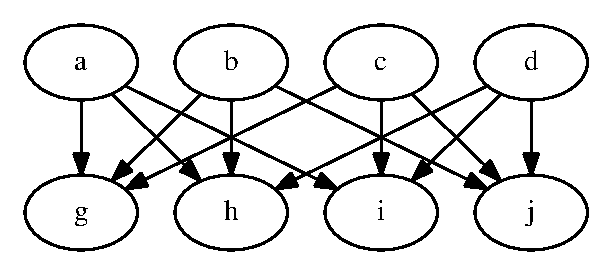
\includegraphics[scale=0.6]{graphs_isomorph_example_1}
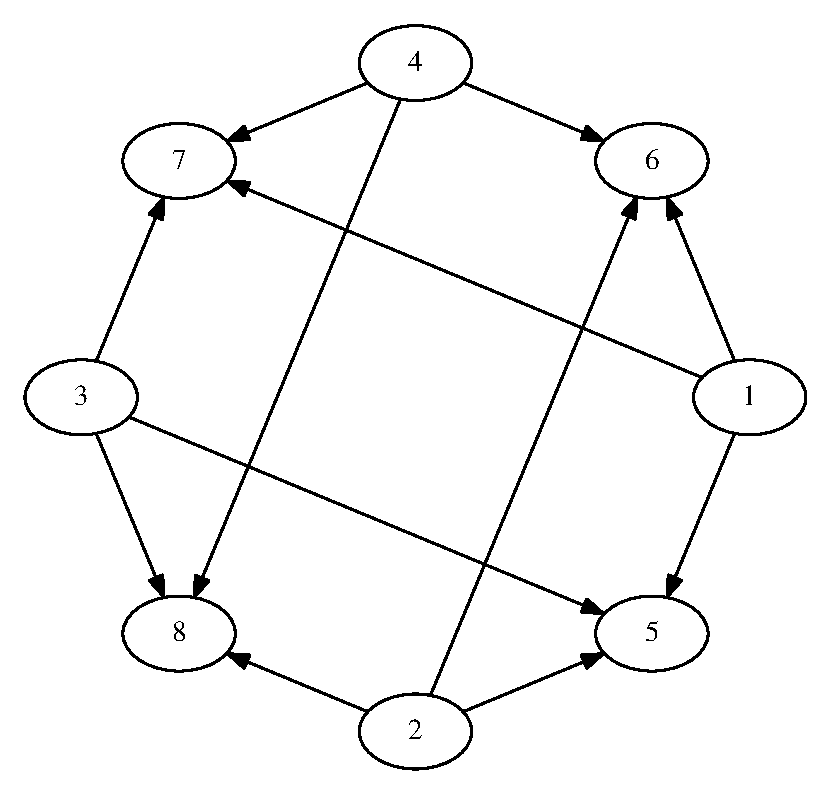
\includegraphics[scale=0.6]{graphs_isomorph_example_2}
\caption{Пример изоморфных графов}
\label{fig:graphs_isomorph_example}
\end{figure}

Пример изоморфных графов представлен на рисунке~\ref{fig:graphs_isomorph_example}.

\textbf{Матрица смежности графа $G$ с конечным числом вершин $n$} - это квадратная матрица $A$ размера $n$, в которой значение элемента $a_{ij}$ равно числу ребер из $i$-й вершины графа в $j$-ю вершину. 

Самый прямолинейный способ установить отношение изоморфности между графами $G$ и $H$ - перестановками строк и столбцов матрицы смежности графа $G$ получить матрицу смежности графа $H$. Однако перебор всех возможных перестановок характеризуется вычислительной сложностью $O(N!)$, что практически исключает применение подобного подхода на практике.

Существует набор числовых характеристик графов, называемыми полными инвариантами\cite{Zukov}, совпадение которых у различных графов является необходимым и достаточным условием изоморфизма. Примерами таких инвариантов являются:
\begin{itemize}
\item Мини-код $\mu_{min}(G)$ матрицы смежности, получаемый путем выписывания двоичных значений матрицы смежности в строчку с последующим переводом полученного двоичного числа в десятичную форму. Мини-коду соответствует такой порядок следования строк и стобцов, при котором полученное значение является минимально возможным.
\item Макси-код $\mu_{max}(G)$ матрицы смежности, получаемый путем выписывания двоичных значений матрицы смежности в строчку с последующим переводом полученного двоичного числа в десятичную форму. Макси-коду соответствует такой порядок следования строк и стобцов, при котором полученное значение является максимально возможным.
\end{itemize}

В настоящее время полный инвариант графа, вычислимый за полиномиальное время, неизвестен, однако не доказано, что он не существует. Попытки его отыскания неоднократно предпринимались в 60-х~--- 80-х годах XX века, однако не увенчались успехом. На данный момент лучший алгоритм определения изоморфизма графов имеет временную оценку сложности $2^{O(\sqrt{n log(n)})}$ \cite{Johnson2005} \cite{BabaiCodenotti2008}.

\subsubsection{Перечень процессов, подлежащих автоматизации}
Процессы, которые подлежат автоматизации:
\begin{enumerate}
\item Генерация первичных алгоритмов проверки изоморфизма графов
\item Эволюционный поиск и отбор наилучших алгоритм проверки изоморфизма графов
\item Качественная оценка полученных алгоритмов проверки изоморфизма графов
\item Визуализация полученных алгоритмов проверки изоморфизма графов
\end{enumerate}

\subsubsection{Выбор и обоснование критериев качества}
Для проектируемой автоматизированной информационной системы приоритетными являются следующие критерии качества:
\begin{itemize}
\item скорость обработки эволюционного процесса
\item используемая память во время обработки эволюционного процесса
\item лицензия на исходный код и исполняемые файлы
\item стоимость приобретения или использования программного продукта
\item используемый язык программирования
\item используемый подход для представления исходного кода алгоритмов
\item удобство работы и документация
\end{itemize}

\textbf{Скорость обработки эволюционного процесса} - однозначно определяется временем, затрачиваемым на обработку одного поколения индивидов при одинаковом количестве запусков на каждого индивида и настройках эволюционных операторов. Данный параметр является самым важным, он определяет насколько быстрее программный продукт найдет качественные решения.

\textbf{Используемая память во время обработки эволюционного процесса} - определяется эффективностью использования адресного пространства ОЗУ вычислительного средства. Меньшее потребление памяти позволяет запускать большее число параллельных популяций для поиска алгоритмов. Является менее важным параметром, так как при плохой скорости обработки преимущество в используемой памяти несущественно.

\textbf{Лицензия на исходный код и исполняемые файлы} - лицензии регулируют правила пользования исходными кодами программы и исполняемыми файлами. Преимущество дают широко распространенные \textbf{свободные} лицензии, котырые позволяют просматривать, модифицировать и распрострянять исходные коды, а к исполняемым файлам прикрепляется инструкция получения исходных кодов. Закрытые (проприетарные) лицензии зачастую используются в платном программном обеспечении, что резко ограничивает его применимость.

\textbf{Стоимость приобретения или использования программного продукта} - многие программные продукты спроектированы для профессионального и/или коммерческого использования, и разработчики данных программ требуют оплату при получении или использовании их программ.

\textbf{Используемый язык программирования} - необходимо разработать АИС на языке программирования \textbf{D}, который является на данный момент современным языком системного и прикладного программирования, ориентированный на создание эффективных понятных и крупных программных комплексов. Пополнение и использование экосистемы языка \textbf{D} является значительным вкладом в развитие области. Для использования других языков с программами, написанными на \textbf{D}, необходимо наличие C-API или специальной обертки, которая пишется программистом под собственные нужды, что означает дополнительные расходы. Поэтому системы, написанные на других языках и которые имеют C-API рассматриваются как более удобные, чем без данного интерфейса взаимодействия.

\textbf{Используемый подход для представления исходного кода алгоритмов} - различные системы генетического программирования используют различные способы представления исходного кода алгоритмов. Для решения рассматриваемой задачи древовидный подход оценивается как самый удобный, так как в процессе эволюции создаются целые алгоритмы, что отличает генетическое программирование от генетических алгоритмов и похожих методов.

\textbf{Удобство работы и документация} - для работы с автоматизированными информационными системами, являющимися научными инструментами, необходимы общирная документация и удобство работы, чтобы обеспечить наискорейшее получение результатов. 

\begin{table}
\centering
\caption{Принятые значения весовых коэффициентов}
\label{tab:quality_koeff}
\begin{tabular}{c|c|c}
Коэффициент & Значение & Описание \\ 
\hline 
$K_1$ & 0.2 & Скорость обработки \\ 
\hline 
$K_2$ & 0.1 & Используемая память \\ 
\hline 
$K_3$ & 0.15 & Лицензия \\ 
\hline 
$K_4$ & 0.15 & Стоимость \\ 
\hline 
$K_5$ & 0.3 & Язык программирования \\ 
\hline 
$K_6$ & 0.05 & Представление алгоритма \\ 
\hline 
$K_7$ & 0.05 & Удобство работы и документация 
\end{tabular} 
\end{table}

Итоговые значения весовых коэффициентов для метода базового критерия представлены в таблице~\ref{tab:quality_koeff}. Необходимое для метода базового критерия нормировки соблюдено:
$$
\sum_i K_i = 1
$$

\subsubsection{Анализ аналогов и прототипов}
Генетическое программирование было заложено Koza, J.R. в \cite{KozaTheBase} в 1992 году. С того времени появилось немало реализаций данного метода, но для сравнения были выбраны самые используемые и широко распространенные.

\paragraph{JGAP} - библиотека, написанная на языке Java, для генетического программирования и генетических алгоритмов. Она предоставляет базовые генетические механизмы, которые могут быть легко использованы в эволюционном подходе для решений задач. JGAP спроектирована простой для использования "из коробки", при этом являясь гибкой системой для того, чтобы пользователи могли легко добавлять свои генетические операторы и другие компоненты.

Документация, качество и стабильность кода являлись главными критериями при проектировании JGAP. Исходный код содержит множество тестов, документирующие комментарии и множество примеров.

Преимущества:
\begin{itemize}
\item Отличная документация и удобство пользования
\item Открытая лицензия
\item Бесплатность
\item Использование необходимой модели внутреннего языка
\end{itemize}

Недостатки:
\begin{itemize}
\item Большое использование памяти (особенность языка)
\item Использование языка, требующего трудоемкой разработки обертки 
\end{itemize}

\paragraph{ECJ} - исследовательская система, написанная на языке Java. Имеет крайне гибкую структуру, где все классы загружаются во время исполнения по заданным пользователем конфигурационным файлам. Также данная система разработана с учетом высокой производительности вычислений.

Преимущества:
\begin{itemize}
\item Высокая скорость обработки
\item Открытая лицензия
\item Бесплатность
\item Использование необходимой модели внутреннего языка
\end{itemize}

Недостатки:
\begin{itemize}
\item Большое использование памяти (особенность языка)
\item Использование языка, требующего трудоемкой разработки обертки 
\item Недостаточный объем документации и примеров
\end{itemize}

\paragraph{ECF} - библиотека, написанная на языке C++, предназначенная для моделирования любого вида эволюционных вычислений. Включает в себя широкий набор методов эволюционных оптимизаций, многопоточное исполнение, хорошо конфигурируемый процесс эволюции.

Преимущества:
\begin{itemize}
\item Высокая скорость обработки
\item Открытая лицензия
\item Бесплатность
\end{itemize}

Недостатки:
\begin{itemize}
\item Использование языка, требующего разработки обертки 
\item Недостаточный объем документации и примеров
\item Используется неудобный способ представления алгоритмов
\end{itemize}

\paragraph{Discipulus} - коммерческая система генетического программирования. Предположительно написанна на C\#, заявляется удобство представления входных данных, интеллектуальная система настройки эволюционного процесса и встроенная защита от проблемы, называемой <<переобучение>>.

Преимущества:
\begin{itemize}
\item Имеет C-API, не нужна разработка обертки
\item Заявляется удобство использования, отсутствующее у конкурентов
\end{itemize}

Недостатки:
\begin{itemize}
\item Платность
\item Проприетарная лицензия
\item Недостаточный объем документации и примеров
\item Мало информации о системе
\end{itemize}

\paragraph{Самостоятельно разработанная АИС} - использован языке программирования \textbf{D}, используется гибкая система, позволяющая заменять любой компонет системы и добавлять свои генетические операции. Предусмотрено множество параметров системы, которые доступны для регулирования пользователем. Система разработана с учетом необходимости высокой производительности и низкого потребления памяти.

Преимущества:
\begin{itemize}
\item Высокая скорость обработки
\item Низкое потребление памяти
\item Написана на целевом языке, не требует оберток
\item Открытая лицензия
\item Бесплатность
\item Большой объем документации различных видов
\end{itemize}

Недостатки:
\begin{itemize}
\item Проблемы со стабильность из-за малого срока разработки
\item Узкая заточенность под конкретную задачу
\end{itemize}

Перевод качественных параметров в количественные производится при помощи таблицы~\ref{tab:quality_to_value}.
\begin{table}
\centering
\caption{Таблица перевода качественных параметров в количественные}
\label{tab:quality_to_value}
\begin{tabular}{|c|c|c|c|c|}
\hline 
Качественное значение & Отлично & Хорошо & Удовлетворительно & Плохо \\ 
\hline 
Количественное значение & 1 & 0.8 & 0.5 & 0.2 \\ 
\hline 
\end{tabular} 
\end{table}

Сперва сравним аналоги без учета весовых коэффициентов, результат сравнения представлен в таблице~\ref{tab:analog_compare_phase1}. Приведенные и нормированные значения количественных критериев с учетом весовых коэффициентов представлены в таблице~\ref{tab:analog_compare_phase2}.

\begin{table}
\centering
\caption{Сравнение аналогов без перевода в количественные значения}
\label{tab:analog_compare_phase1}
\begin{tabular}{c|c|c|c|c|c}
Критерий & JGAP & ECJ & ECF & Discipulus & Данная АИС \\ 
\hline 
$K_1$ & Отлично & Хорошо & Отлично & Хорошо & Хорошо \\ 
\hline 
$K_2$ & Удовл. & Удовл. & Хорошо & Хорошо & Хорошо \\ 
\hline 
$K_3$ & Отлично & Отлично & Отлично & Удовл. & Отлично \\ 
\hline 
$K_4$ & Отлично & Отлично & Отлично & Плохо & Отлично \\ 
\hline 
$K_5$ & Удовл. & Удовл. & Хорошо & Хорошо & Отлично \\ 
\hline 
$K_6$ & Отлично & Отлично & Хорошо & Хорошо & Отлично \\ 
\hline 
$K_7$ & Отлично & Удовл. & Удовл. & Плохо & Хорошо 
\end{tabular} 
\end{table}

\begin{table}
\centering
\caption{Сравнение аналогов и прототипов с учетом нормировки и весовых коэффициентов}
\label{tab:analog_compare_phase2}
\begin{tabular}{c|c|c|c|c|c|c}
Критерий & $\alpha$ & JGAP & ECJ & ECF & Discipulus & Данная АИС \\ 
\hline 
$K_1$ & 0.2 & 1.0 & 0.8 & 1.0 & 0.8 & 0.8 \\ 
\hline 
$K_2$ & 0.1 & 0.5 & 0.5 & 0.8 & 0.8 & 0.8 \\ 
\hline 
$K_3$ & 0.15 & 1.0 & 1.0 & 1.0 & 0.5 & 1.0 \\ 
\hline 
$K_4$ & 0.15 & 1.0 & 1.0 & 1.0 & 0.2 & 1.0 \\ 
\hline 
$K_5$ & 0.3 & 0.5 & 0.5 & 0.8 & 0.8 & 1.0 \\ 
\hline 
$K_6$ & 0.05 & 1.0 & 1.0 & 0.8 & 0.8 & 1.0 \\ 
\hline 
$K_7$ & 0.05 & 1.0 & 0.5 & 0.5 & 0.2 & 0.8 \\ 
\hline 
$\sum_i \alpha_i K_i$ & 1.0 & 0.8 & 0.735 & 0.885 & 0.635 & 0.93  
\end{tabular} 
\end{table}

Из произведенных расчетов видно, что разработка собственной информационной автоматизированной системы является целесообразным, так как она соответствует поставленным целям лучше, чем существующие аналоги.

\newpage
\subsection{Разработка программного изделия}
\subsubsection{Разработка структуры программного изделия}
АИС состоит из нескольких подсистем и разбита на две большие части:
\begin{itemize}
\item Внутренняя часть, которая разрабатывалась специально под решаемую задачу в рамках данной работы. Модули, относящиеся к этой части, будем называть \textbf{внутренние}. 
\item Внешняя часть - модули, относящиеся к библиотеке генетического программирования \textbf{Devol}, разработанной ранее как многофункциональное инструментальное средство для генетического программирования. Изначально \textbf{Devol} являлся коллективной разработкой (автор является одним из основных разработчиков), и в рамках данной работы эта библиотека была переработана и дополнена, чтобы отвечать поставленным целям. Данные модули будем называть \textbf{внешние}.
\end{itemize}

Графическая схема модулей АИС представлена на листе~2 графической части и на рис.~\ref{fig:modulesScheme}.

\begin{figure}[h!]
\centering

\includegraphics[width=1.0\textwidth]{modules}
\caption{Схема модулей АИС}
\label{fig:modulesScheme}
\end{figure}

\subsubsection{Описание модулей программного изделия}
Внутренние модули АИС:
\begin{itemize}
\item \textbf{main} - главный модуль системы, точка входа приложения. В нем инициализируются объект приложения, все окна и логгер
\item \textbf{application} - описание класса приложения, хранит ссылки на все окна, логгер, проект и управляет механизмом завершения работы приложения
\item \textbf{project} - описание сохраняемых параметров АИС. Сохранению подлежат: параметры эволюции, имя популяции и популяция
\item \textbf{gui} - пакет, который содержит подпакеты, относящиеся к графическому интерфейсу пользователя:
\begin{itemize}
\item \textbf{evolution} - описание окна эволюции
\item \textbf{generic} - описание общего поведения для всех окон, включая главное меню
\item \textbf{results} - описание окна результатов
\item \textbf{settings} - описание окна настроек эволюции и просмотра проблемно - ориентированного языка
\item \textbf{util} - содежрит алгоритм переключения между окнами
\end{itemize}
\item \textbf{graph} - пакет, содержащий подпакеты, относящиеся к реализации ориентированных графов:
\begin{itemize}
\item \textbf{connectivity} - реализация ориентированного графа на списках связности
\item \textbf{directed} - описание интерфейса ориентированного графа
\end{itemize}
\item \textbf{evol} - пакет, содержащий подпакеты, относящиеся к эволюционным процессам:
\begin{itemize}
\item \textbf{compiler} - описание стратегии компиляции, параметризация популяции и интерпретатора проблемно-ориентированного языка
\item \textbf{individ} - описание алгоритма распознавания изоморфизма графов как инидивида в популяции
\item \textbf{progtype} - описание настроек эволюционного процесса, также загружает все операторы и типы проблемно-ориентированного языка
\item \textbf{world} - описание среды, в которой выполняются программы-индивиды. Описание функции приспособленности и генерации входных графов
\item \textbf{operators} - пакет, содержащий подпакеты, относящиеся к операторам проблемно-ориентированного языка:
\begin{itemize}
\item \textbf{and} - описание оператора логического "И"
\item \textbf{answer} - описание оператора записи ответа на поставленную задачу
\item \textbf{construct} - описание создание аргумента, описывающего ребро графа
\item \textbf{dist} - описание получения индекса конца ребра графа
\item \textbf{div} - описание арифметического оператора деления
\item \textbf{gdup} - описание операции над стеком общего назначения: дублирование вершины стека
\item \textbf{gover} - описание операции над стеком общего назначения: копирование аргумента под вершиной стека и расположение копии на вершине
\item \textbf{gpop} - описание операции над стеком общего назначения: снятие значения с вершины стека
\item \textbf{gpush} - описание операции над стеком общего назначения: сохранение аргумента в стеке
\item \textbf{grot} -  описание операции над стеком общего назначения: перемещение третьего с вершины аргумента в стеке на вершину
\item \textbf{gswap} - описание операции над стеком общего назначения: перемещение вершины стека под следующий за ней аргумент
\item \textbf{idcast} -  описание оператора преобразования целочисленной переменной в действительную
\item \textbf{idup} - описание операции над входными стеками: дублирование вершины стека
\item \textbf{iover} - описание операции над входными стеками: копирование аргумента под вершиной стека и расположение копии на вершине
\item \textbf{ipop} - описание операции над входными стеками: снятие значения с вершины стека
\item \textbf{ipush} - описание операции над входными стеками: сохранение аргумента в стеке
\item \textbf{irot} -  описание операции над входными стеками: перемещение третьего с вершины аргумента в стеке на вершину
\item \textbf{iswap} - описание операции над входными стеками: перемещение вершины стека под следующий за ней аргумент
\item \textbf{mult} - описание арифметического оператора умножения
\item \textbf{not} -  описание оператора логичекого "НЕ"
\item \textbf{opif} - описание оператора логического вевтления
\item \textbf{opwhile} - описание оператора цикла
\item \textbf{or} - описание оператора логического "ИЛИ"
\item \textbf{plus} - описание оператора арифметического сложения
\item \textbf{relation} - описание операторов сравнения: больше, меньше, больше равно, меньше равно
\item \textbf{round} - описание оператора округления, преобразования действительного аргумента к целочисленному
\item \textbf{source} - описание получения индекса начала ребра графа
\end{itemize}
\item \textbf{types} - пакет, содержащий подпакеты, относящиеся к описанию типов проблемно-ориентированного языка:
\begin{itemize}
\item \textbf{argedge} - описание аргумента, содержащего ребро графа
\item \textbf{typedge} - описание типа ребра графа
\end{itemize}
\end{itemize}
\end{itemize}

Внешние модули АИС, используемые во внутренних модулях:
\begin{itemize}
\item \textbf{devol.compiler} - описание общих процедур интерпретации программ-индивидов
\item \textbf{devol.population} - описание популяции-контейнера, параметризируемого пользовательским типом инидивидов
\item \textbf{devol.individ} - описание базовой абстракции индивида-программы, перегружаемой пользователем
\item \textbf{devol.std.argvoid} - описание аргумента "нулевого" типа
\item \textbf{devol.programtype} - описание необходимых параметров, которые должен предоставить пользователь для работы эволюционного процесса
\item \textbf{devol.operatormng} - менеджер операторов, хранящий в себе все операторы проблемно-ориенитированного языка
\item \textbf{devol.operator} - базовое описание оператора, которое должен перегружать пользователь для создания своих операторов
\item \textbf{devol.std.typepod} - описание типа, содержащего простые типы данных
\item \textbf{devol.std.argpod} - описание аргумента, содержащего значения простых типов данных
\item \textbf{devol.world} - базовое описание окружения, которое пререгружается пользователем
\item \textbf{devol.argument} - описание аргумента, хранящего значения некоторого типа
\item \textbf{devol.type} - описание типа, используемого в операторах проблемно-ориенитрованного языка
\item \textbf{devol.serializable} - интерфейс, стандартизирующий операции сохранения/загрузки
\item \textbf{devol.typemng} - менеджер типов, хранящий все типы, используемые в проблемно-ориентированном языке
\end{itemize}

\subsubsection{Особенности выбранных технологий}
Все компоненты АИС написаны на языке программирования \textbf{D}, используются следующие зависимости:
\begin{itemize}
\item gtk-d - привязки к библиотеке графических элементов GTK+
\item dyaml - пакет, реализующий операции сохранения и загрузки и/в формат YAML
\item devol - разработанный автором пакет для генетического программирования
\end{itemize}

\subsubsection{Язык програмирования D}
\textbf{D} — объектно-ориентированный, императивный, мультипарадигмальный язык программирования, созданный Уолтером Брайтом из компании Digital Mars. Изначально был задуман как переработка языка C++, однако, несмотря на значительное влияние С++, не является его вариантом. В D были заново реализованы некоторые свойства C++, также язык испытал влияние концепций из других языков программирования, таких как Java, Python, Ruby, C\# и Eiffel.

При создании языка D была сделана попытка соединить производительность компилируемых языков программирования с безопасностью и выразительностью динамических. Код на языке D обычно работает так же быстро как эквивалентный код на C++, при этом программа на D короче и обеспечивает безопасный доступ к памяти.

D является мультипарадигменным языком и поддерживает в полной мере следующие парадигмы:
\begin{itemize}
\item процедурно-структурное программирование
\item объектно-ориентированное программирование
\item функциональное программирование
\item контрактное программирование
\item обобщенное программирование
\end{itemize}

D получает все большую популярность из-за преимуществ над предшественником C++. Развитая система обобщенного программирования с переосмысленными шаблонами и примесями вместе с интроспекцией дает мощный инструмент для создания эффективных и гибких приложений, работающих под разными платформами. В D присутствует выполенение функций на этапе компиляции, что позволяет "программировать" компилятор и определять свои проблемно-ориентированные языки.

D используеют сборщик мусора, который можно отключить для тех частей приложения, для которых необходимо ручное управление памятью. 

Объектно-ориентированная парадигма языка D является продолжателем идей, заложенных в С++ и развитых в языке Java, но имеет свои особенности. Так, например, классы передаются в функции только по ссылке, без изначально заложенной возможности копирования по значению. В языке отсутствует множественное наследование классов, но имеется множественное наследование интерфесов.

\subsubsection{Язык разметки YAML}
\textbf{YAML} — человекочитаемый формат сериализации данных, концептуально близкий к языкам разметки, но ориентированный на удобство ввода-вывода типичных структур данных многих языков программирования. Используется в АИС для сохранения информации о проекте.

\subsubsection{Библиотека графических элементов GTK+}
\textbf{GTK+} (сокращение от GIMP ToolKit) — кроссплатформенная библиотека элементов интерфейса, имеет простой в использовании API, наряду с Qt является одной из двух наиболее популярных на сегодняшний день библиотек для X Window System. Используется в АИС для построения графического интерфейса пользователя.

\subsubsection{Архитектруа программы. UML-диаграмма классов}
Во время проектирования приложения были выбраны следующие директивы:
\begin{itemize}
\item Максимальная гибкость. Архитектура приложения должна поддерживать легкое изменение практически всех компонентов, включая добавление и удаление новых типов и операторов проблемно-ориентированного языка
\item Максимальная эффективность. Используя богатые возможности языка D, программа должна выполняться как можно быстрее и потреблять как можно меньше памяти, при этом не терять в гибкости и скорости разработки
\item Минимальные издержки. Все операции, которые могут быть проведены и верифицированы на этапе компиляции, должны быть перемещены на этап компиляции. Критически важные алгоритмы должны быть протестированы встроенными модульными тестами.
\end{itemize}

Классы, используемые в АИС, можно разделить на 3 типа:
\begin{itemize}
\item Ядро - классы, обеспечивающие описание графов, приложения и логики сохранения/загрузки информации
\item Графический интерфейс - классы, описывающие графический интерфейс пользователя
\item Эволюционные - описание внутреннего проблемно-ориентированного языка генетического программирования
\item Внешние - используемые зависимости и классы библиотеки Devol
\end{itemize}

Диаграмма классов изображена на листе 6 графической части и на рис.~\ref{fig:classDiagram}.

\begin{figure}[h!]
\centering
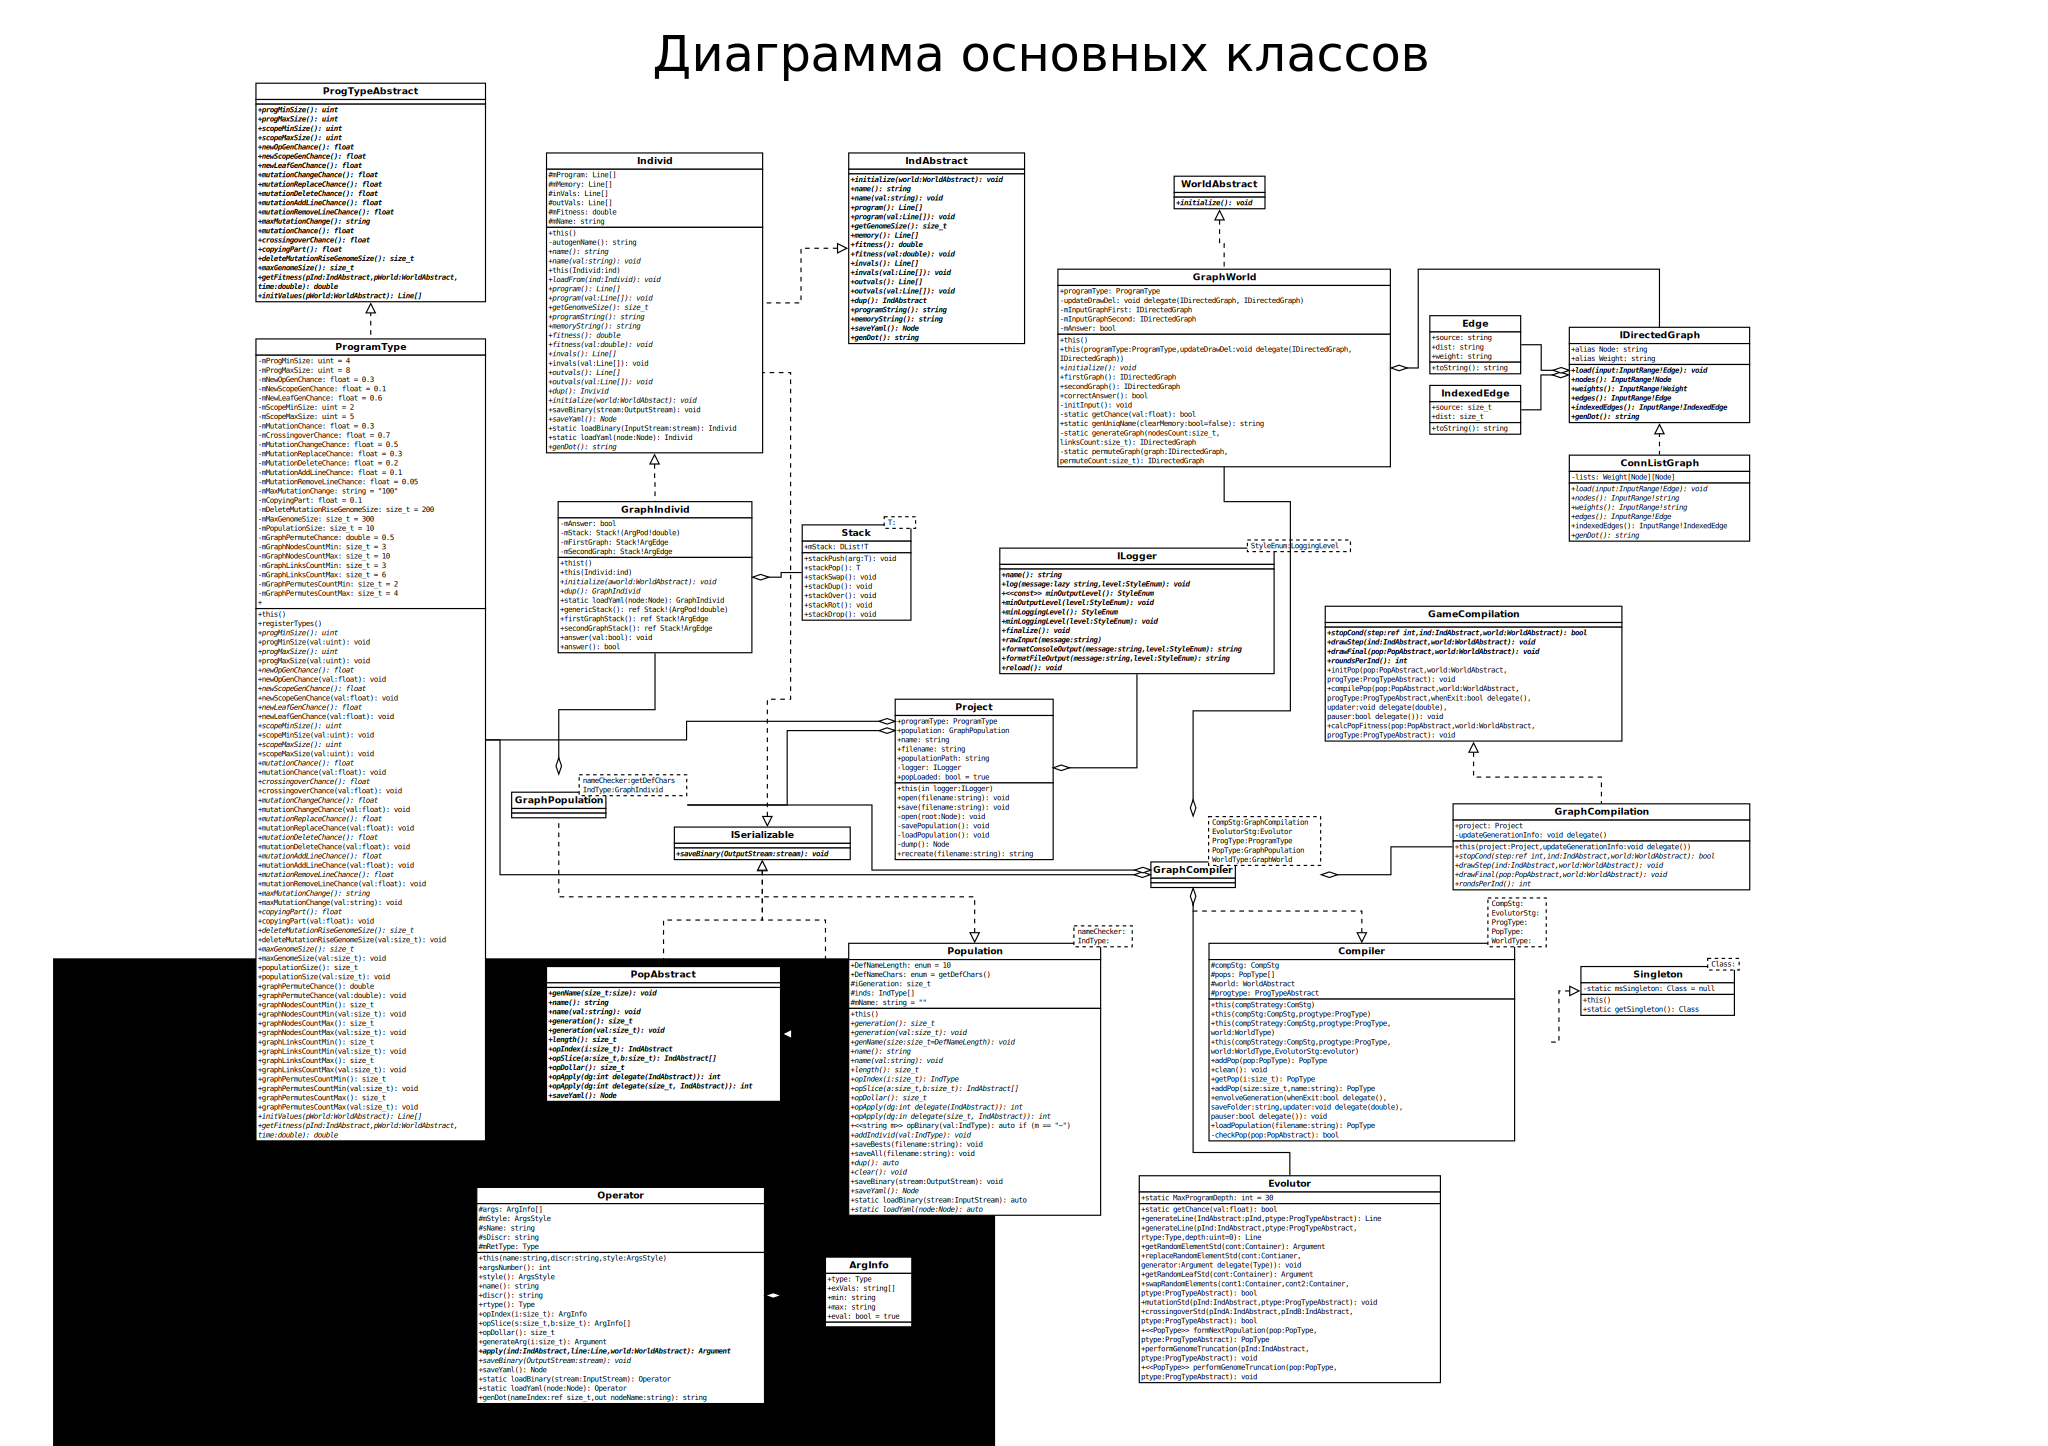
\includegraphics[width=1.3\textwidth, angle=90]{list6}
\caption{Диаграмма основных классов АИС}
\label{fig:classDiagram}
\end{figure}

Перечень классов:
\begin{itemize}
\item \textbf{Application} - содержит проект и все окна приложения, определяет алгоритмы инициализации и завершения работы приложения
\item \textbf{Project} - проект, хранящий все параметры эволюционного процесса, имя популяции и последнюю найденную популяцию
\item \textbf{EvolutionWindow} - окно эволюции, в котором отображается процесс эволюции
\item \textbf{GenericWindow} - хранит в себе общее поведение для всех окон, включая главное меню
\item \textbf{ResultsWindow} - окно результатов, в котором отображаются индивиды текущей популяции
\item \textbf{SettingsWindow} - окно настроек эволюции, где пользователь может просмотреть используемые операторы и настроить процесс эволюции
\item \textbf{IDirectedGraph} - интерфейс, описывающий ориентированный граф
\item \textbf{ConnListGraph} - реализация ориентированного графа на основе списков смежности
\item \textbf{GraphWorld} - описание окружения исполнения алгоритмов проверки изоморфизма, отвечает за генерацию входных графов
\item \textbf{ProgramType} - описание параметров эволюционного процесса, все настройки эволюции находятся в этом классе
\item \textbf{GraphIndivid} - описание алгоритма проверки изоморфизма графов как индивида в популяции. Каждый индивид содержит в себе три стека:
\begin{itemize}
\item Стек общего назначения с действительным типом элементов
\item Первый входной стек для первого графа
\item Второй входной стек для второго графа
\end{itemize}
\item \textbf{GraphPopulation} - контейнер для индивидов, параметризированный типом GraphIndivid
\item \textbf{GraphCompilation} - описание правил компиляции индивидов и популяций. Является наследником GamePopulation, использующий раундовый метод определения итогового значения функции приспособленности.
\item \textbf{GraphCompiler} - интерпретатор алгоритмов в терминах проблемно-ориентированного языка для популяций GraphIndivid со стандартными алгоритмами мутации, кросинговера, нахождения нужных поддеревьев над типизированными деревьями.
\item \textbf{TypeEdge} - описание типа ребра графаф для внутреннего языка, является упорядоченной парой индексов вершин
\item \textbf{ArgEdge} - описание контейнера для значения типа ребра графа
\item \textbf{AndOperator} - описание оператора логического "И"
\item \textbf{AnswerOperator} - описание оператора записи ответа на поставленную задачу
\item \textbf{ConstructOperator} - описание создание аргумента, описывающего ребро графа
\item \textbf{DistOperator} - описание получения индекса конца ребра графа
\item \textbf{DivOperator} - описание арифметического оператора деления
\item \textbf{GenericDupOperator} - описание операции над стеком общего назначения: дублирование вершины стека
\item \textbf{GenericoverOperator} - описание операции над стеком общего назначения: копирование аргумента под вершиной стека и расположение копии на вершине
\item \textbf{GenericpopOperator} - описание операции над стеком общего назначения: снятие значения с вершины стека
\item \textbf{GenericpushOperator} - описание операции над стеком общего назначения: сохранение аргумента в стеке
\item \textbf{GenericrotOperator} -  описание операции над стеком общего назначения: перемещение третьего с вершины аргумента в стеке на вершину
\item \textbf{GenericswapOperator} - описание операции над стеком общего назначения: перемещение вершины стека под следующий за ней аргумент
\item \textbf{IntDoubleCastOperator} -  описание оператора преобразования целочисленной переменной в действительную
\item \textbf{InputDupFirstOperator, InputDupSecondOperator} - описание операции над входными стеками: дублирование вершины стека
\item \textbf{InputOverFirstOperator, InputOverSecondOperator} - описание операции над входными стеками: копирование аргумента под вершиной стека и расположение копии на вершине
\item \textbf{InputPopFirstOperator, InputPopSecondOperator} - описание операции над входными стеками: снятие значения с вершины стека
\item \textbf{InputPushFirstOperator, InputPushSecondOperator} - описание операции над входными стеками: сохранение аргумента в стеке
\item \textbf{InputRotFirstOperator, InputRotSecondOperator} -  описание операции над входными стеками: перемещение третьего с вершины аргумента в стеке на вершину
\item \textbf{InputSwapFirstOperator, InputSwapSecondOperator} - описание операции над входными стеками: перемещение вершины стека под следующий за ней аргумент
\item \textbf{MultOperator} - описание арифметического оператора умножения
\item \textbf{NotOperator} -  описание оператора логичекого "НЕ"
\item \textbf{IfOperator} - описание оператора логического вевтления
\item \textbf{WhileOperator} - описание оператора цикла
\item \textbf{OrOperator} - описание оператора логического "ИЛИ"
\item \textbf{PlusOperator} - описание оператора арифметического сложения
\item \textbf{IntEqualOperator} - описание оператора равенства целочисленных значений
\item \textbf{DoubleEqualOperator} - описание оператора равенства действительных значений
\item \textbf{IntGreaterOperator} - описание оператора "больше" для целочисленных значений
\item \textbf{IntLesserOperator} - описание оператора "меньше" для целочисленных значений
\item \textbf{IntGreaterEqualOperator} - описание оператора "больше равно" для целочисленных значений
\item \textbf{IntLesserEqualOperator} - описание оператора "меньше равно" для целочисленных значений
\item \textbf{DoubleGreaterOperator} - описание оператора "больше" для действительных значений
\item \textbf{DoubleLesserOperator} - описание оператора "меньше" для действительных значений
\item \textbf{DoubleGreaterEqualOperator} - описание оператора "больше равно" для действительных значений
\item \textbf{DoubleLesserEqualOperator} - описание оператора "меньше равно" для действительных значений
\item \textbf{RoundOperator} - описание оператора округления, преобразования действительного аргумента к целочисленному
\item \textbf{SourceOperator} - описание получения индекса начала ребра графа
\item \textbf{ProgramTypeAbstract} - базовое описание параметров, которые должны быть заданы для эволюционного процесса
\item \textbf{IndAbstract} - базовое описание индивида, которое должно быть задано для эволюционного процесса
\item \textbf{Individ} - стандартная реализация индивида, которое перегружается пользователем для описания своих индивидов
\item \textbf{WorldAbstract} - базовое описание окружения исполнения индивида
\item \textbf{ILogger} - интерфейс для системы логгирования. Конкретная реализация скрыта за этим интерфейсом.
\item \textbf{GameCompilation} - базовое описание стратегии компиляции "игра"
\item \textbf{Singleton} - описание свойств объекта, который существует только в одном экземпляре
\item \textbf{Evolutor} - содержит описание эволюционных алгоритмов
\item \textbf{PopAbstract} - базовое описание контейнера для инидвидов
\item \textbf{Operator} - описание класса-базы для задания операторов проблемно-ориентированного языка
\item \textbf{ArgInfo} - описание аргумента оператора
\item \textbf{Stack}  - описание стеков, хранящихся внутри индивида
\item \textbf{Edge} - ребро графа
\item \textbf{IndexedEdge} - ребро графа, где исходные вершины заменены на индексы, непосредственно используется операторами языка
\end{itemize}

\subsubsection{Выбор программных средств}

\paragraph{Выбор операционной системы для разработки программного продукта}
Изначально АИС разрабатывалась для использования в окружении операционной системы GNU/Linux, но так как при проектировании не были использованы платформозависимые возможности языка и не использованы зависимости, имеющие только одну основную платформу, то данный продукт должен работать и под другими платформами: MacOS, Windows, семейство BSD. Необходимым условием является наличие компилятора языка D и реализации библиотеки GTK+.

\paragraph{Выбор системы спопровождения разработки}
В качестве системы сборки и пакетного менеджера использовался пакетный менеджер \textbf{Dub}, который на данный момент является безальтернативным практически стандартным средством для управления пакетами на D. В качестве системы контроля версий была выбрана \textbf{git} и репозиторий на домене \textbf{gighub.com}, так как это основной способ публикации пакетов в \textbf{Dub registry} - оффициальный регистр пакетов для языка программирования D.

\paragraph{Выбор среды разрабоки программного продукта}
Разработка велась в окружении операционной системы GNU/Linux, в которой в качестве IDE практически безальтернативно является \textbf{Eclipse} с плагином \textbf{Descent} для разработки на языке программирования D. Кроссплатформенность, интеграция с пакетным менеджером \textbf{Dub}, бесплатность, навигация по коду и интеграция с системами контроля версий делают \textbf{Eclipse} очевидным выбором. 

\subsubsection{Выбор аппаратных средств}
АИС предназначена для работы на компьютерах одной из архитектур: x86, x86\underline{~}64. Минимальные характеристики, необходимые для работы:
\begin{itemize}
\item Процессор, поддерживающий архитектуру x86\underline{~}64 с тактовой частотой не менее 1.5 ГГц
\item Оперативная память от 1 Гб
\item Графический ускоритель и монитор, способные отображать графический интерфейс операционной системы
\item Устройства ввода: мышь и клавиатура
\end{itemize}

\subsubsection{Разработка основных алгоритмов обработки информации}
АИС использует широкий спект нетривиальных алгоритмов:
\begin{itemize}
\item Алгоритм типизированной мутации
\item Алгоритм типизированного кроссинговера
\item Алгоритм генерации типизированного дерева
\item Алгоритм получения новой популяции
\item Алгоритм выбора случайного узла дерева
\end{itemize}

\subsubsection{Типизированная мутация}
Операция состоит из двух частей:
\begin{itemize}
\item глобальная мутация:
\begin{itemize}
\item добавление новой линии в геном 
\item удаление линии из генома
\end{itemize}
\item локальная мутация:
\begin{itemize}
\item изменение значения аргумента
\item замена листа дерева
\item удаление узла
\end{itemize}
\end{itemize}

Алгоритм использует функцию броска кубика с заданными вероятностями для каждой грани:
$$
k = randomRange([chance_1, chance_2, chance_3])
$$
Значение $k$ будет равно $0$ с вероятностью $chance_1$, $1$ с вероятностью $chance_2$, $2$ с вероятностью $chance_3$.

При попытке удаления узла с типом $void$ необходимо генерировать новую линию, так как простой аргумент пустого типа является исключительной ситуацией и не несет никакой информации, полезной для решения задачи.

\clearpage
\begin{figure}[h!]
\centering
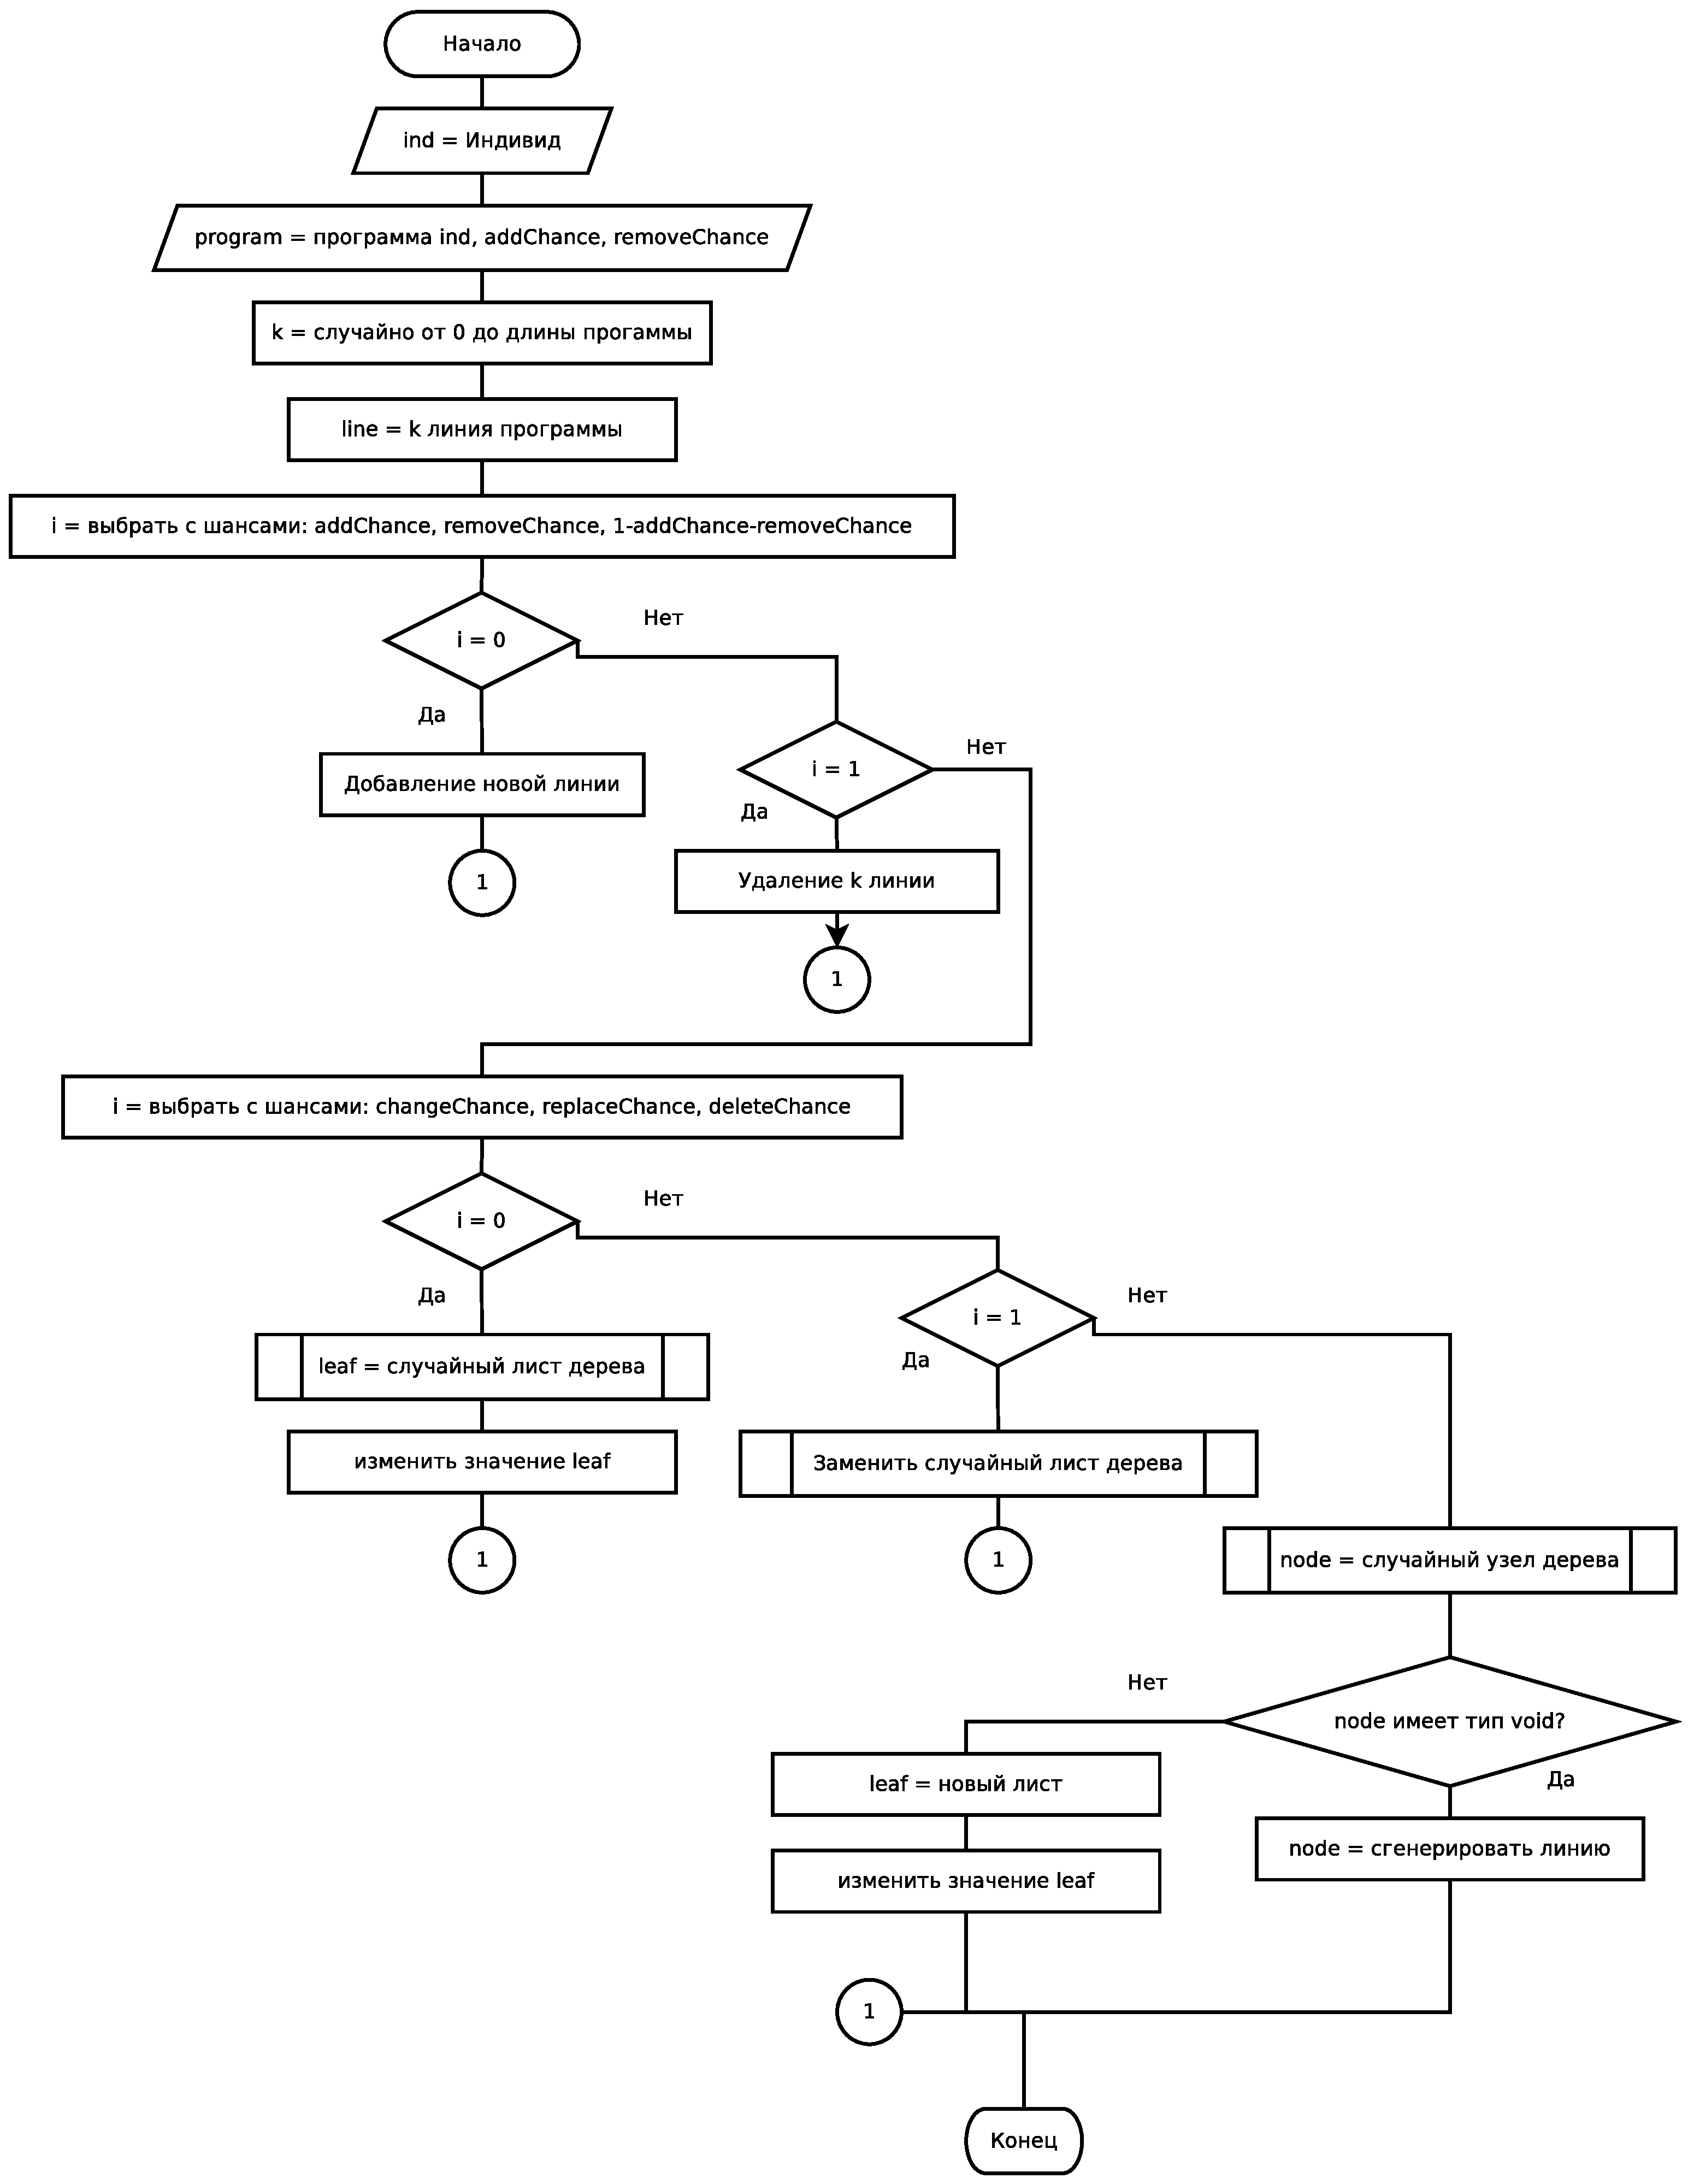
\includegraphics[height=0.85\textheight]{mutation_alg.eps}
\end{figure}
\newpage

\subsubsection{Типизированный кроссинговер}
Используемый алгоритм кроссинговера относится к гибридному подходу: одновременно идет обмен целыми линиями генома и обмен поддеревьями определенных линий. Но шанс обмена целыми линиями обратно пропорционален количеству узлов в деревьях. Это необходимо для обеспечения равномерности распределения выбора узлов дерева для кроссиновера.
\clearpage
\begin{figure}[h!]
\centering
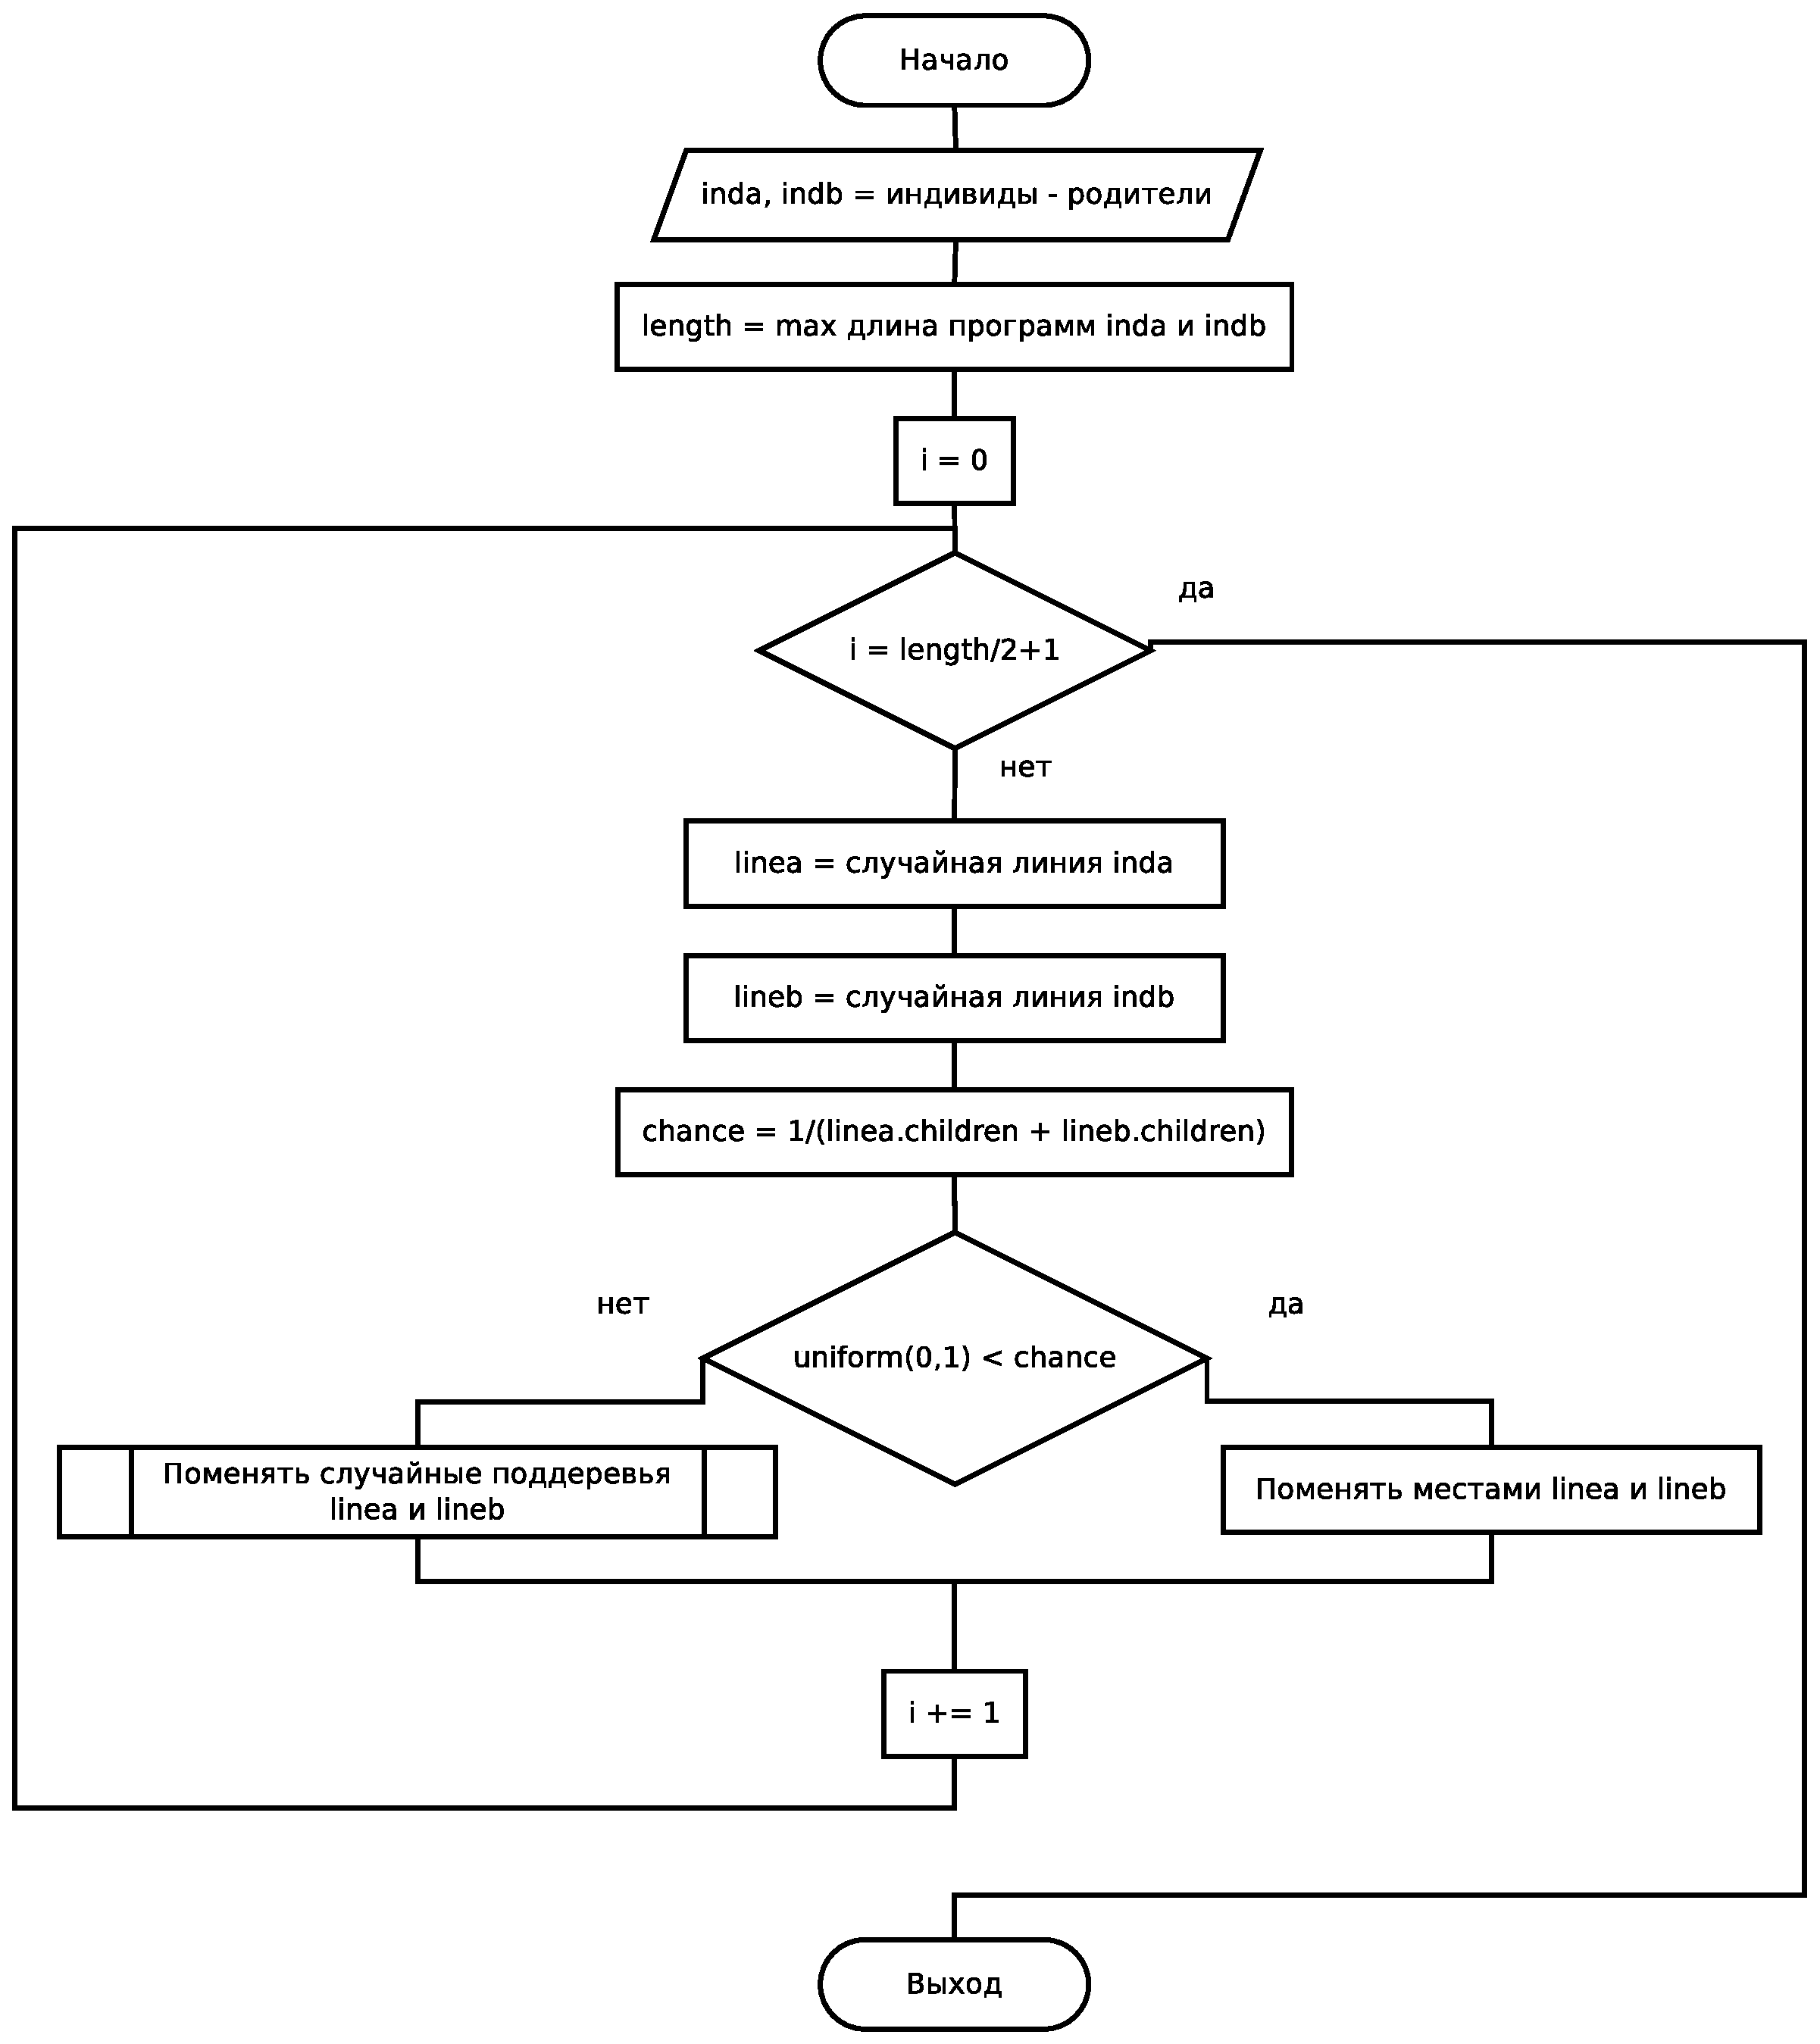
\includegraphics[width=0.9\textwidth]{crossingover_alg.eps}
\end{figure}
\newpage

\subsubsection{Генерация типизированного дерева}
Алгоритм состоит из двух больших частей:
\begin{itemize}
\item генерация нетипизированной линии для корневой области
\item генерация типизированной линии для соблюдения строгой типизации
\end{itemize}
При генерации аргумента с пустым типом возможны два сценария:
\begin{itemize}
\item генерация линии, тип оператора которой определяется аргументом, для которого проводится генерация
\item генерация области с размером от scopeMinSize до scopeMaxSize (задается пользователем)
\end{itemize}
Алгоритм является рекурсивным и останавливается либо самостоятельно из-за генерации констант, либо из-за генерации деревьев максимальной глубины. Специальное ограничение на глубину необъодимо, так как нельзя заранее сказать какой глубины будет сгененрировано дерево (может закончиться доступная память), тем более параметры данной генерации задаются пользователем.

\clearpage
\begin{figure}[h!]
\centering
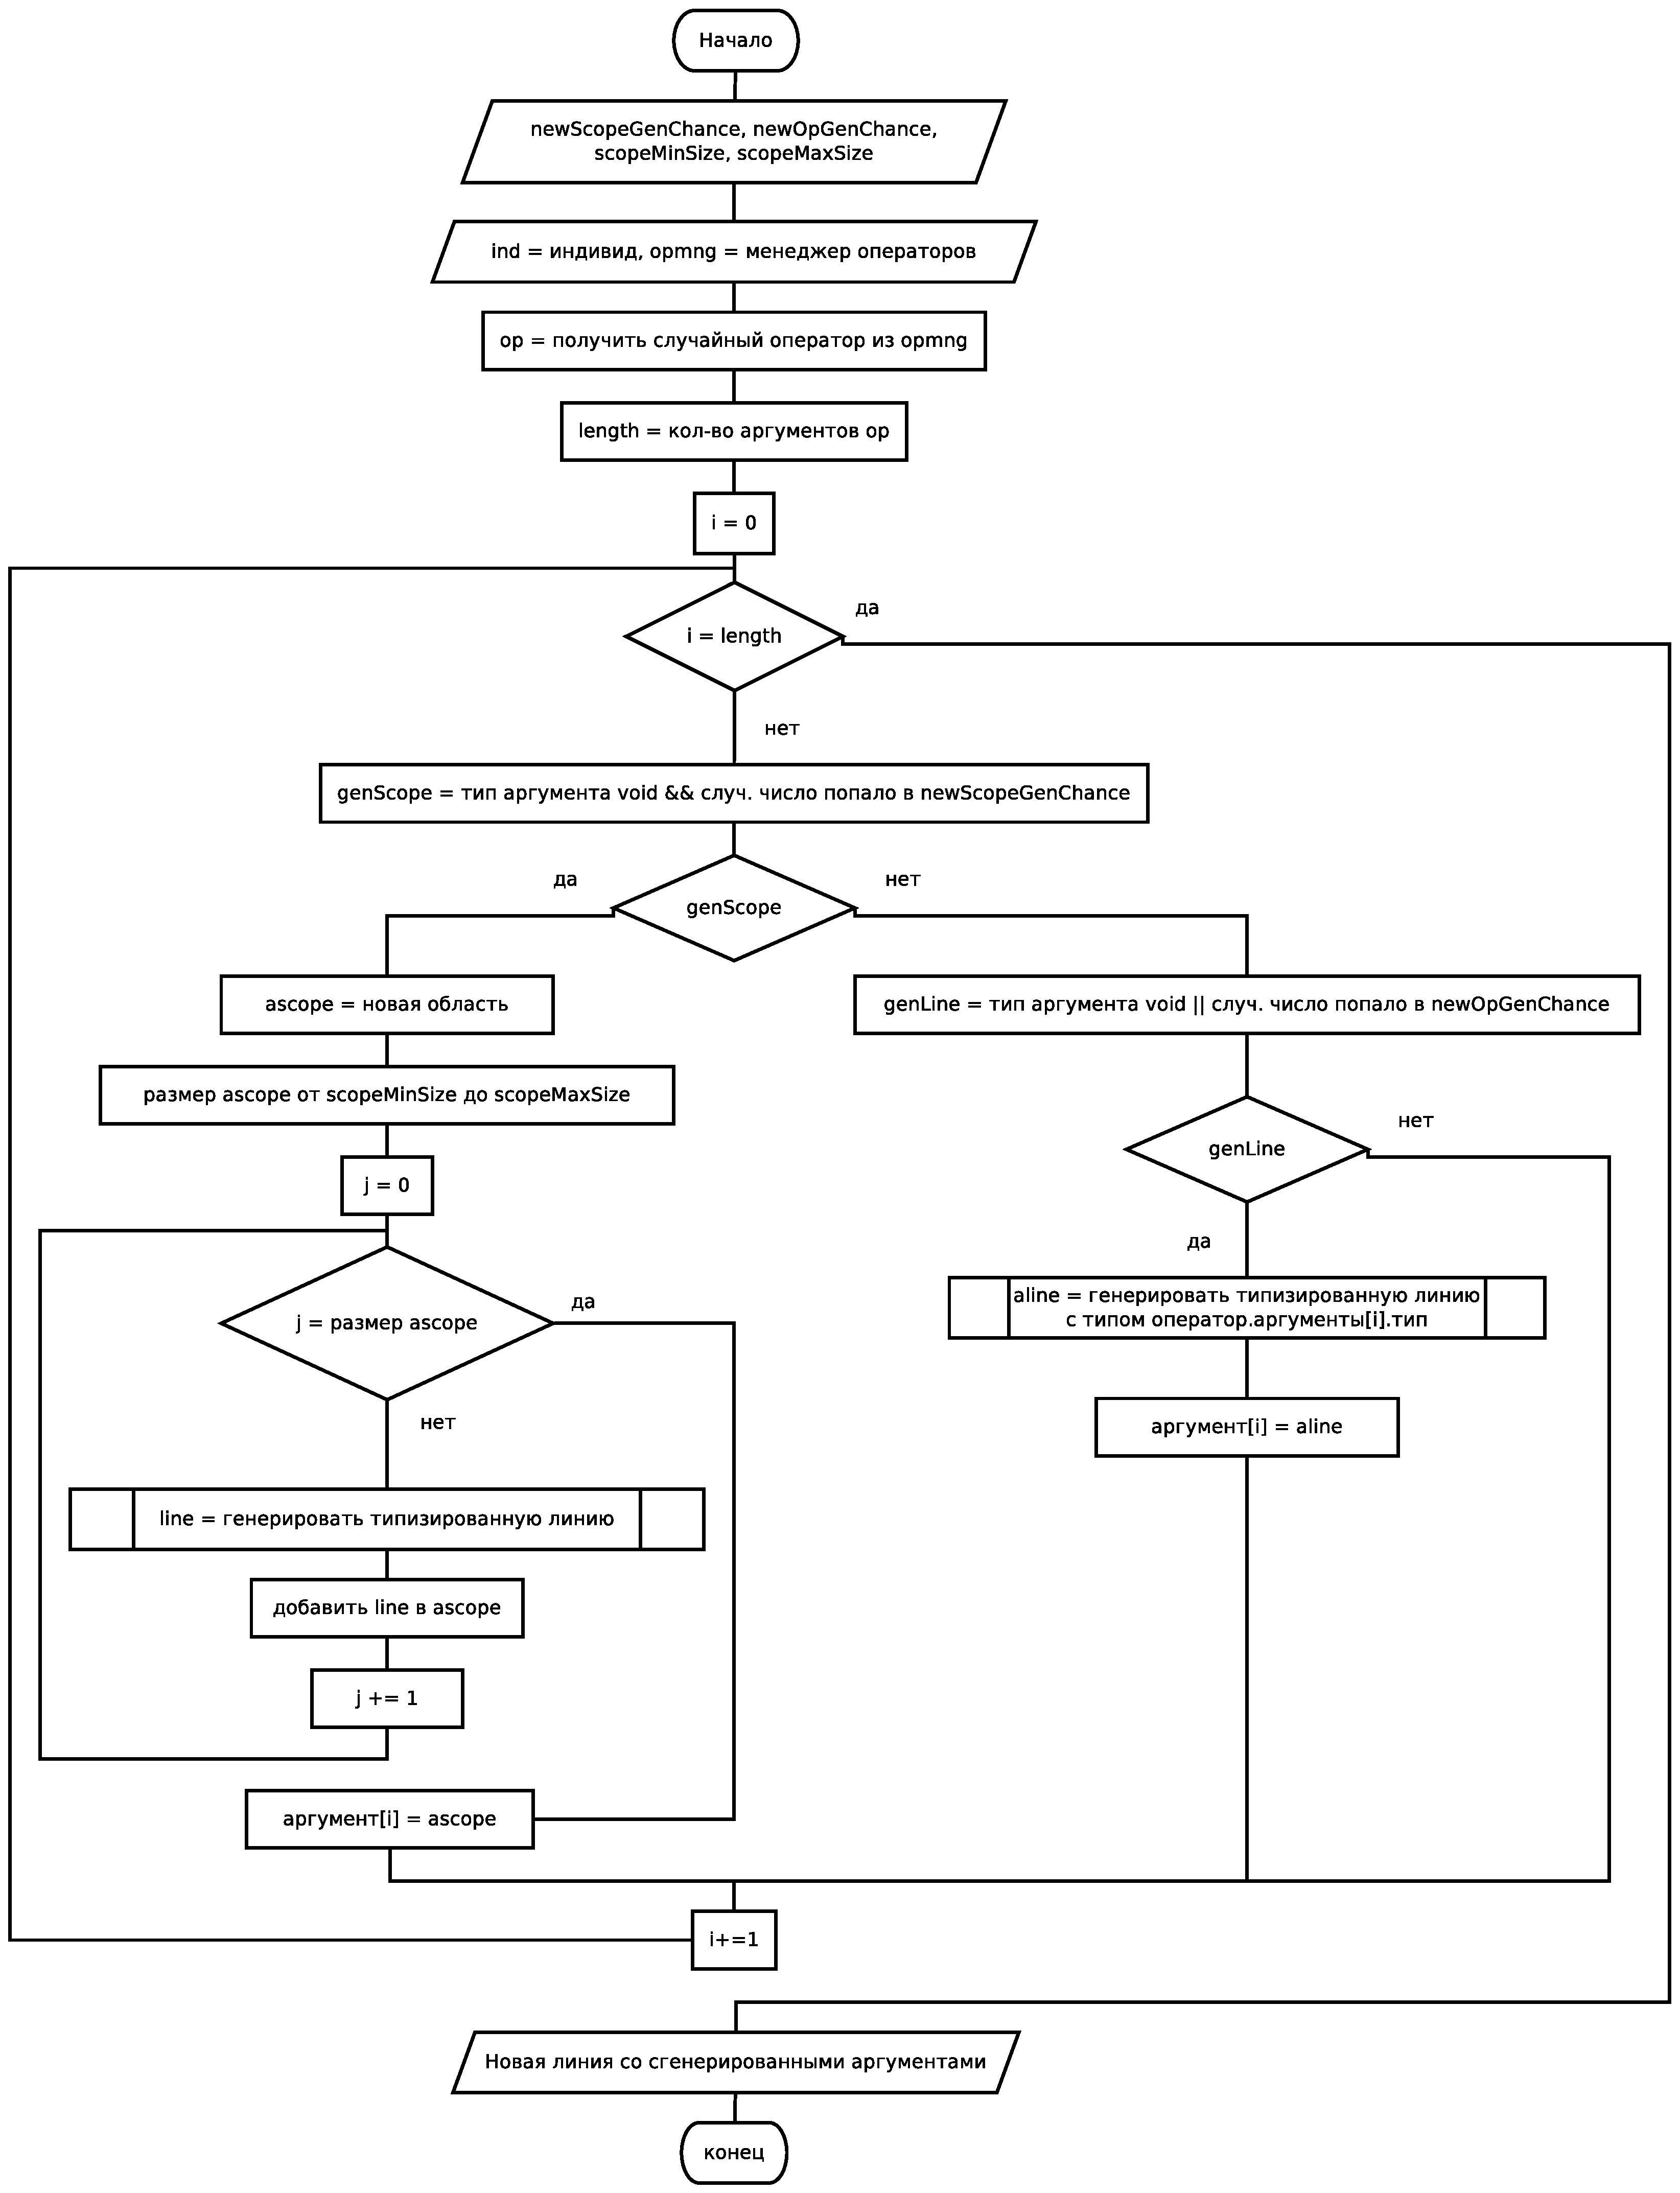
\includegraphics[width=1.0\textwidth]{generate_line_alg.eps}
\end{figure}

\clearpage
\begin{figure}[h!]
\centering
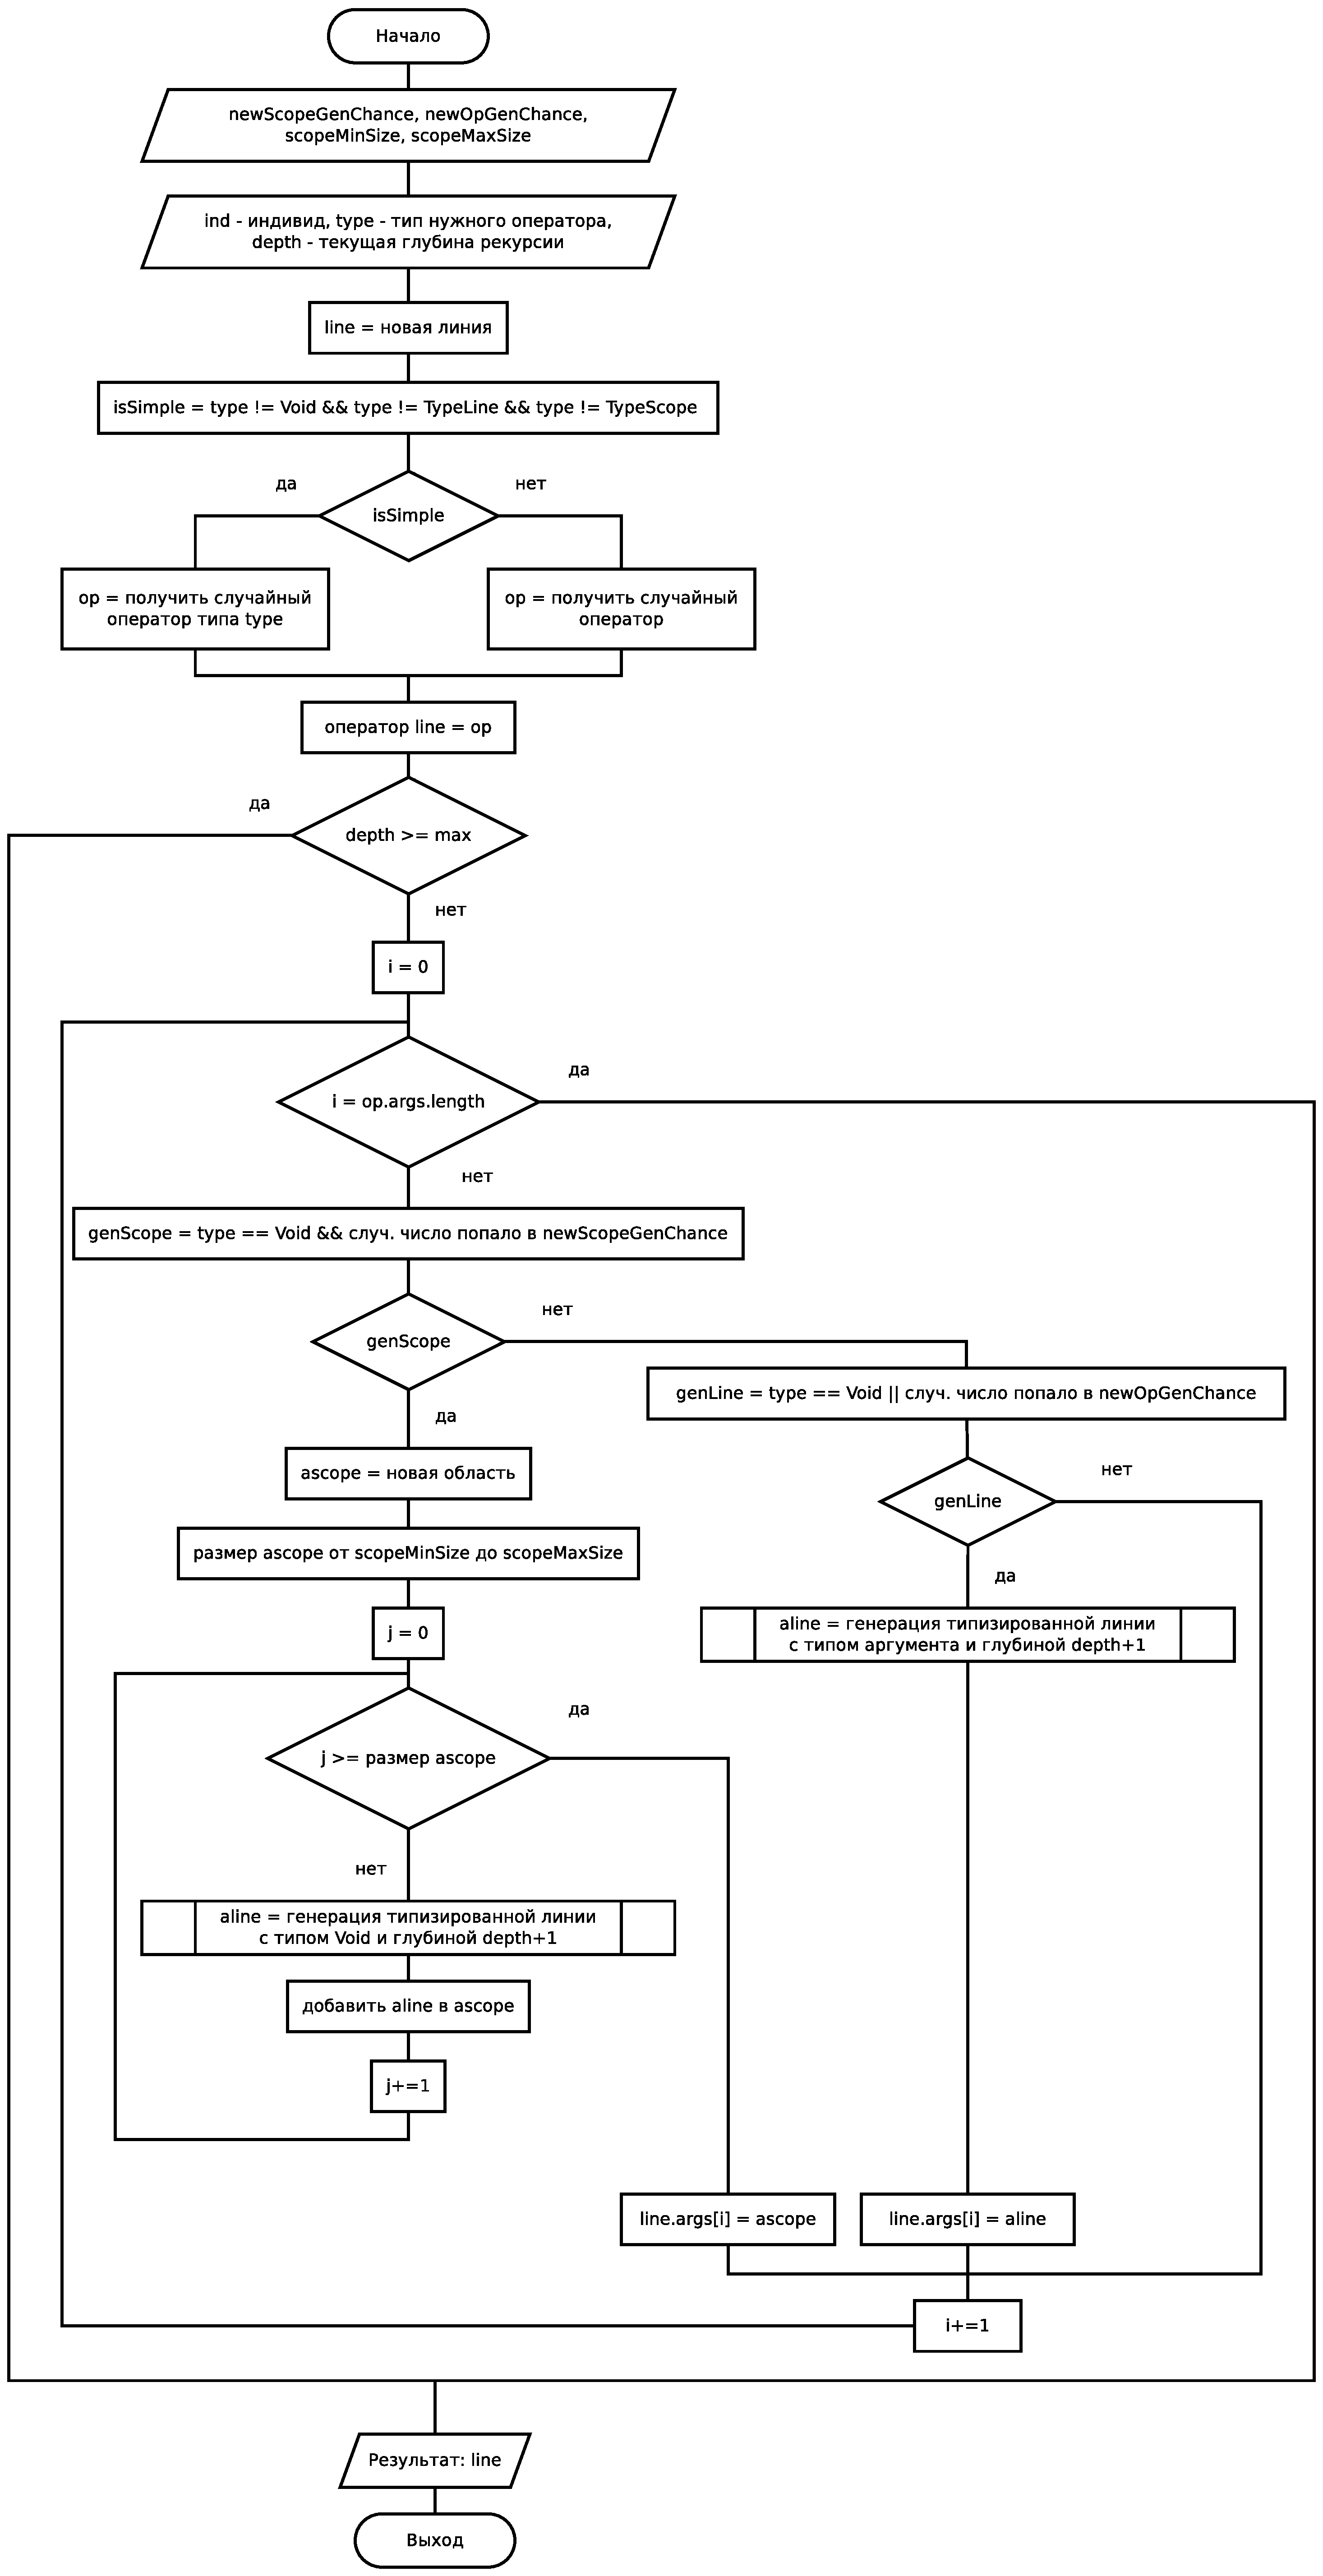
\includegraphics[height=1.0\textheight]{generate_typed_line_alg.eps}
\end{figure}
\clearpage

\newpage
\subsubsection{Получение новой популяции}
В АИС используется практически классический подход при генерации новой популяции. Сначала индивиды сортируются по убыванию функции приспособленности и в новую популяцию попадает часть лучших (copyingPart, задается пользователем), этот прием копирования "элитных" геномов позволяет избежать деградации популяции. Далее расчитывается среднее значение функции приспособленности, на основе которого рассчитываются вероятности каждого индивида для генетических операций (алгоритм нормализует массив вероятностей):
$$
P_i = \frac{f_i}{f_{max}}
$$

В соответствии с вероятностью каждого индивида и шансом операции выполняются либо операция мутации, либо кроссинговер. Обработанные индивиды заполняют новую популяцию. Нужно учитывать, что при нечетном размере популяции один из последних индивидов должен отбрасываться, чтобы избежать утечки памяти.

\clearpage
\begin{figure}[h!]
\centering
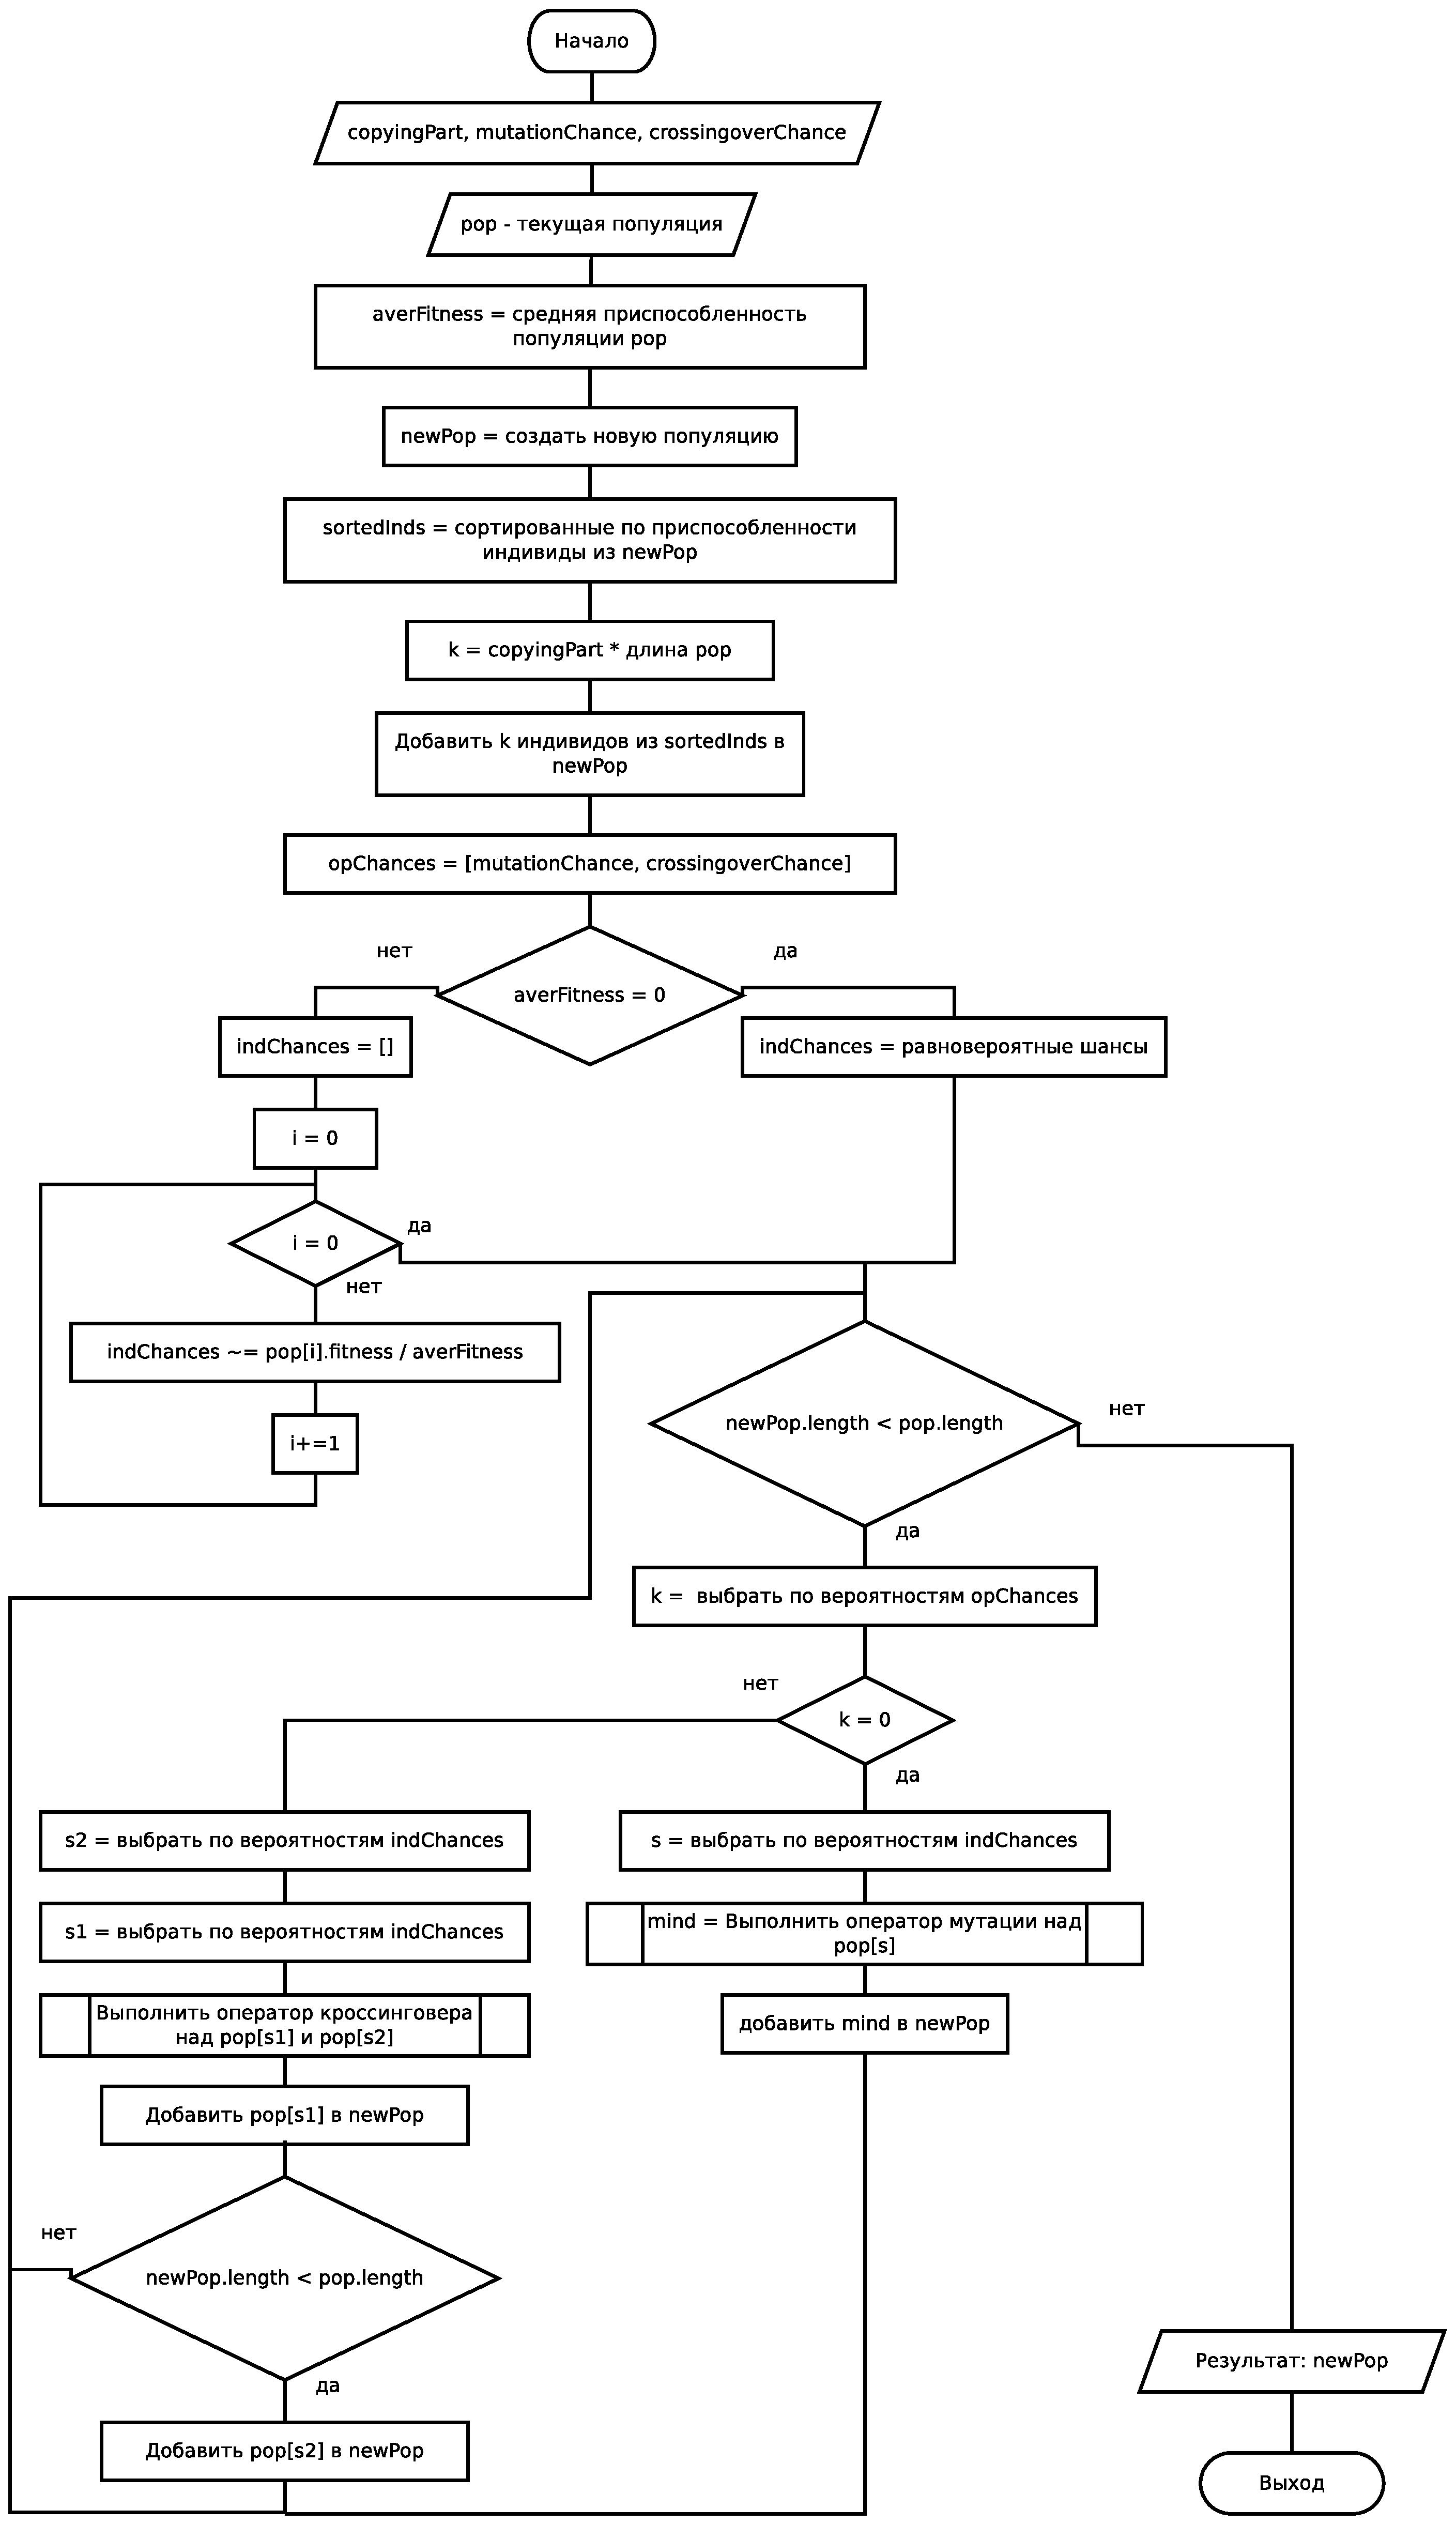
\includegraphics[height=0.9\textheight]{form_next_population_alg.eps}
\end{figure}
\newpage

\subsubsection{Выбор случайного узла дерева}
Данный алгоритм производит выбор узла дерева с равномерным распределением. Для того, чтобы реализовать требование равномерности, расчет вероятности выбора элемента и перехода на уровень вглубь рассчитываются в зависимости от количество потомков дерева.
Вероятность выбрать данный узел:
$$
p_0 = \frac{1}{tree.childs}
$$
Вероятность выбрать $i$-ый аргумент:
$$
p_i = \frac{arg_i.childs}{tree.childs}
$$
Алгоритм останавливается, когда достигается лист или выбирается один из узлов.

\clearpage
\begin{figure}[h!]
\centering
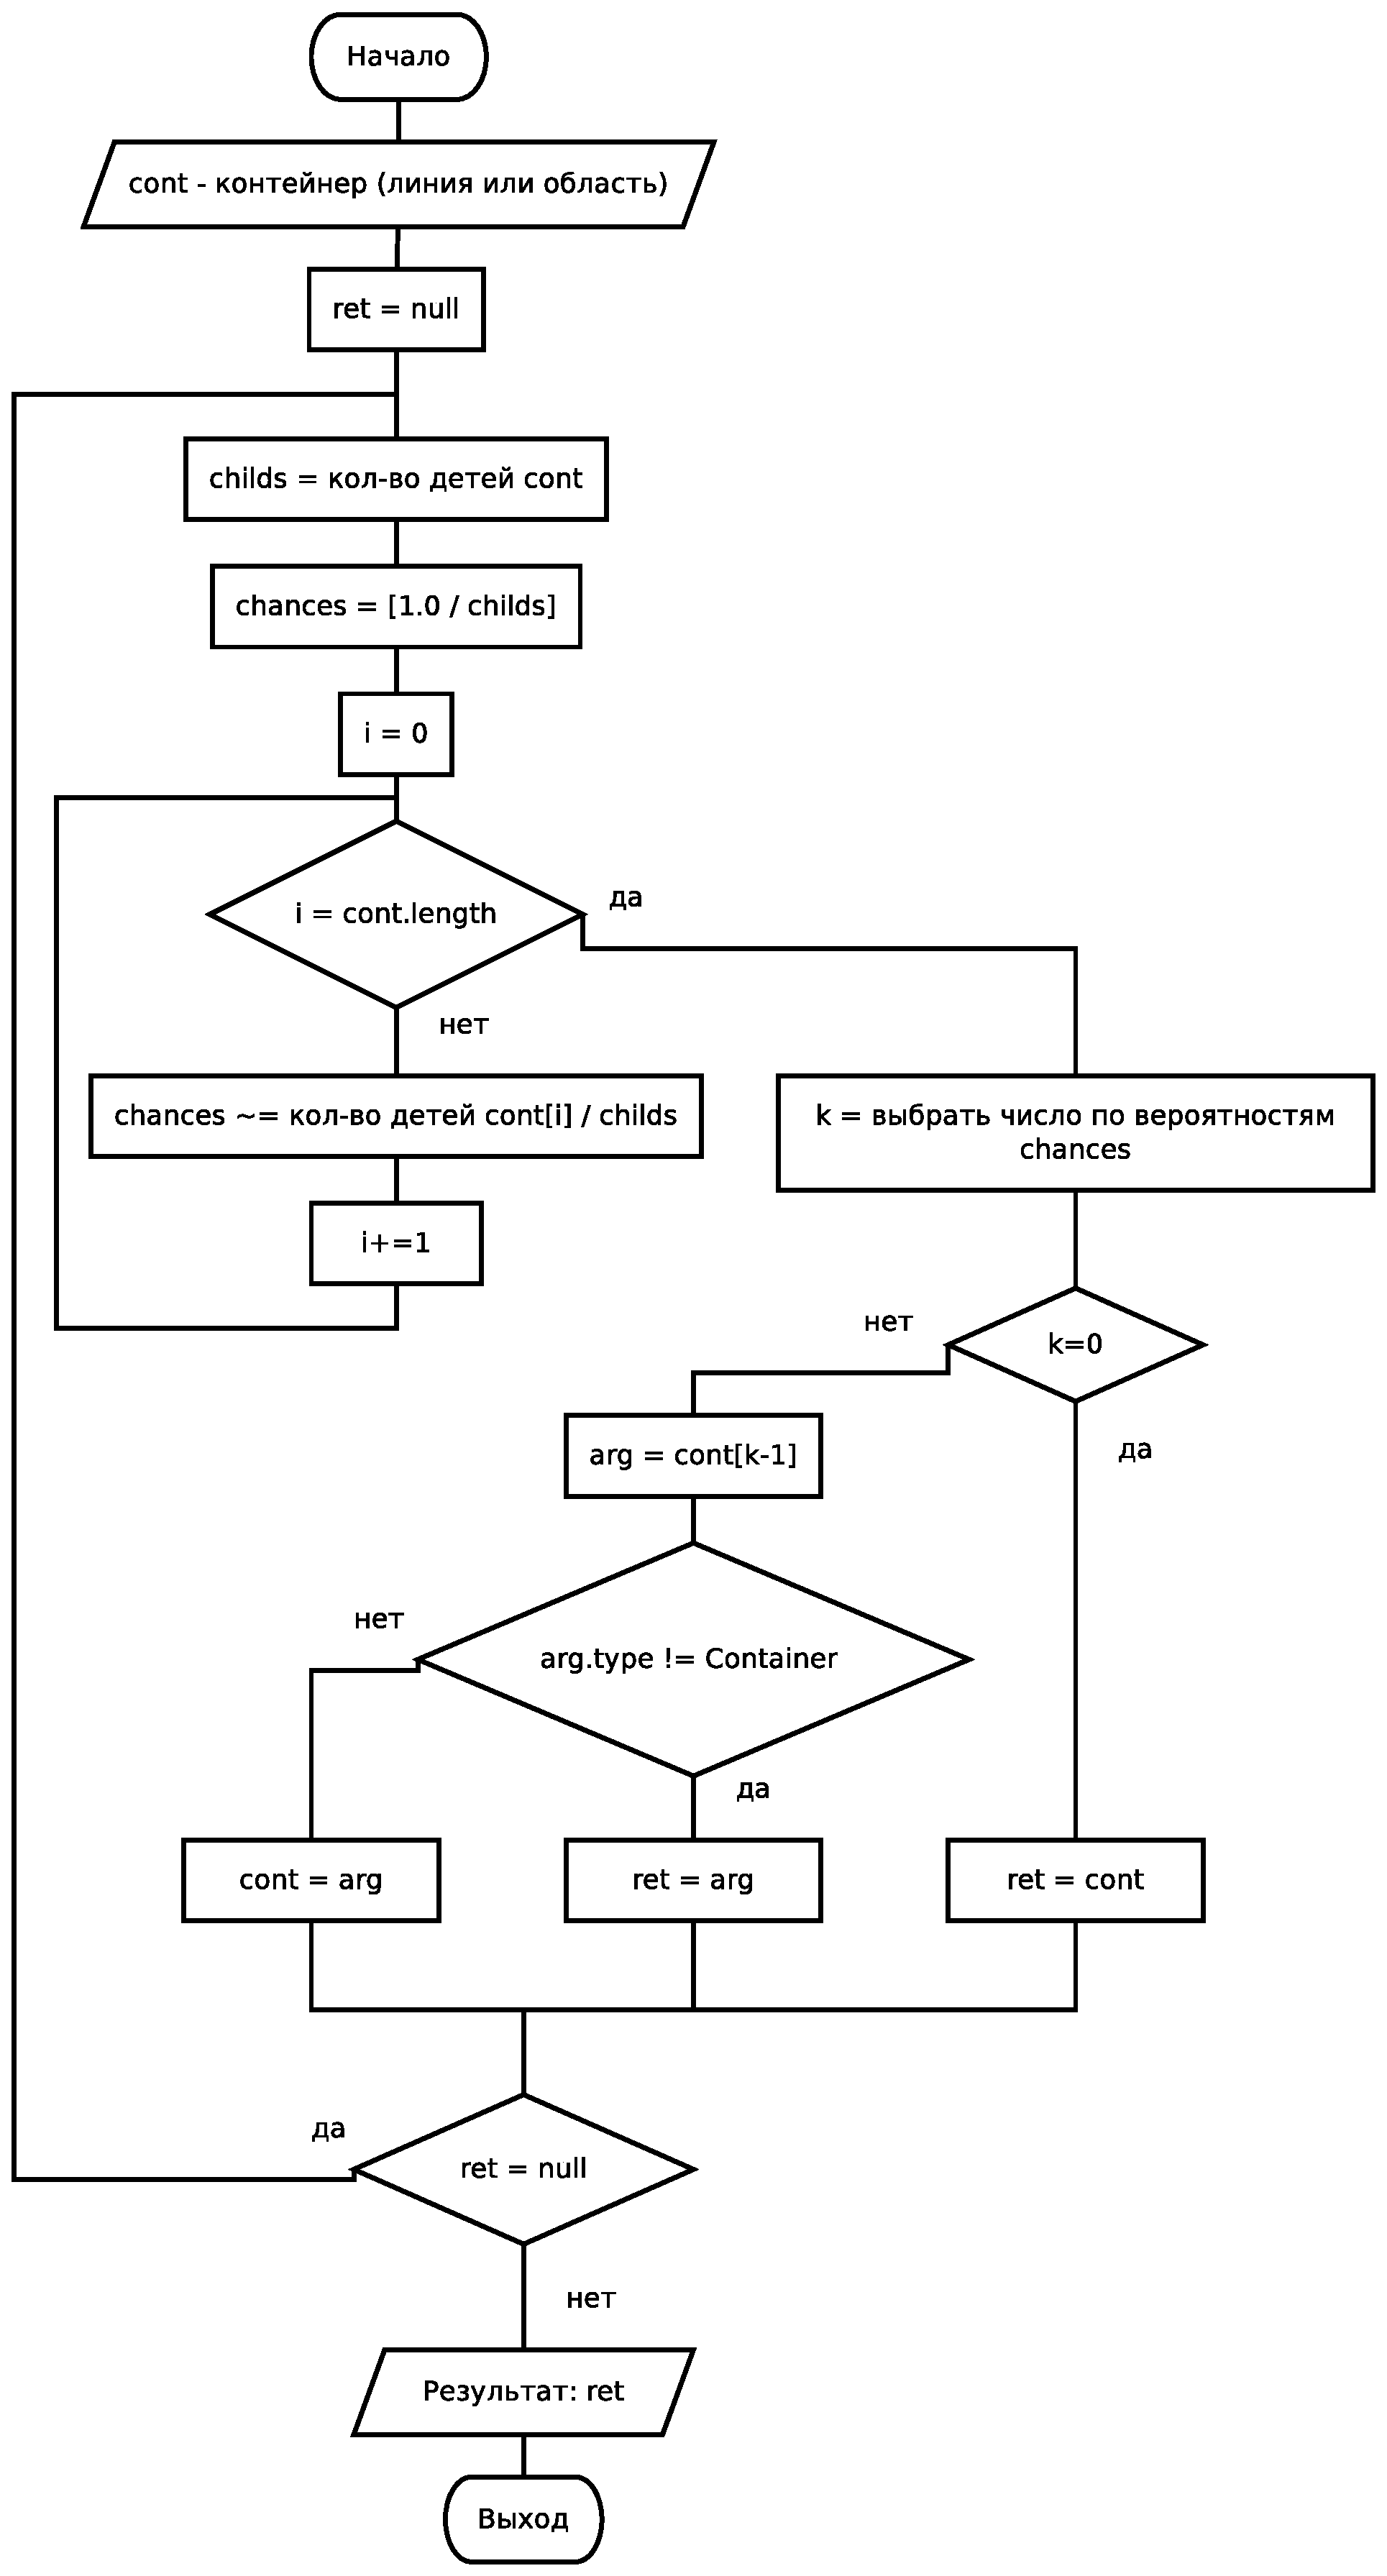
\includegraphics[height=0.9\textheight]{get_random_element_alg.eps}
\end{figure}

\newpage
\subsection{Технологическая часть}
\subsection{Разработка интерфейса взаимодействия с пользователем}
Целью данного этапа является разработка удобного и простого интерфейса, который позволяет пользователю работать с АИС с максимальной продуктивностью.

Графический интерфейс пользователя разрабатывался в конструкторе графических интерфейсов пользователя \textbf{Glade} для \textbf{GTK+}. Для удобства представления и ввода данных были разработы три экранных формы, каждая из которых отвечает за свою часть требований технического задания:
\begin{itemize}
\item Экранная форма настроек эволюционного процесса. Через нее осуществляется просмотр операторов проблемно-ориентированного языка и задание настроек эволюционного процесса. Предусматривается проверка входных данных на корректность.
\begin{figure}[h!]
\centering
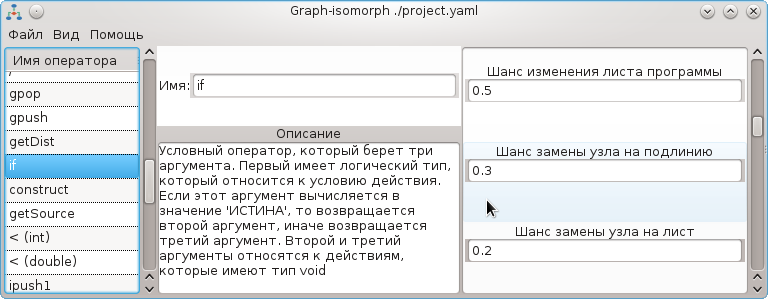
\includegraphics[width=0.8\textwidth]{screen07}
\caption{Графическая форма настроек эволюционного процесса}
\end{figure}

\item Форма управления процессом эволюции. На данной форме отображается статус обработки нового поколения и текущие изображения входных графов для тестируемых алгоритмов.
\begin{figure}[h!]
\centering
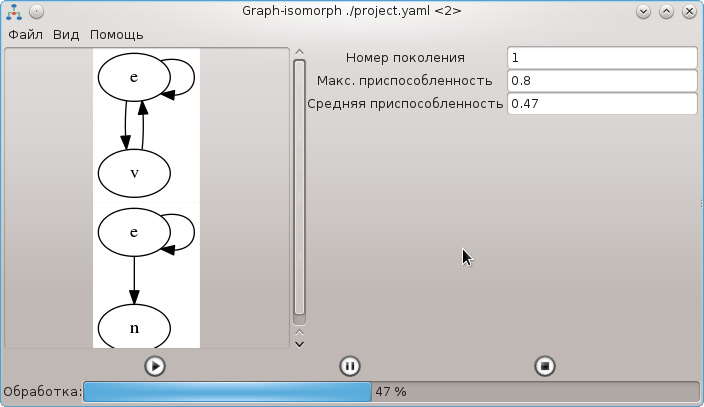
\includegraphics[width=0.8\textwidth]{screen09}
\caption{Экранная форма управления процессом эволюции}
\end{figure}


\item Форма просмотра результатов эволюции. На данной форме отображаются: состав текущей популяции, текстовое представление исходного кода алгоритма-индивида, графическое представление кода алгоритма-индивида.

\begin{figure}[h!]
\centering
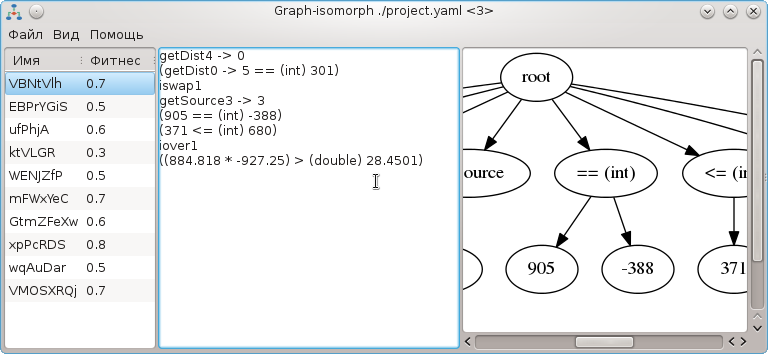
\includegraphics[width=0.8\textwidth]{screen19}
\caption{Экранная форма управления процессом эволюции}
\end{figure}

\end{itemize}

Вывод изображений исходного кода и изображений входных графов осуществляется через систему визуализации графов \textbf{Graphviz}, перед этим алгоритмы проходят специальную обработку для представления их исходного кода в специальной нотации, понятной системе визуализации.

Нужно заметить, что интерфейс программы разрабатывался с учетом возможных изменений его внешнего вида без перекомпиляции программы. Для этого описание интерфейса хранится в отдельном файле с расширением \textbf{.glade}, который загружается при старте приложения, и по информации из этого файла строится внешний вид графического интерфейса пользователя. В программе есть возможность использовать нестандартный путь до файла описания интерфейса, путем передачи своего имени файла при старте приложения через ключ \textbf{--gui}. 

Полный граф диалога с пользователем изображен на рис.~\ref{fig:dialogGraph} и на листе 7 графического приложения.

\begin{figure}[h!]
\centering

\includegraphics[width=1.3\textwidth, angle=90]{list7}
\caption{Граф диалога с пользователем}
\label{fig:dialogGraph}
\end{figure}

\subsection{Разработка форматов входных и выходных данных программы}
\subsubsection{Разработка форм входных данных}

Входные данные программы делятся на два вида:
\begin{itemize}
\item Входные данные, вводимые пользователем через экранные формы. Пользователь, используя графические элементы ввода, предоставляет детальные настройки процесса эволюции.
\item Входные данные, загружаемые из проектного файла. Все введенные пользователем данные сохраняются в так называемом \textbf{проекте}, для возможности продолжить поиск с момента предыдущей остановки эволюционного процесса. Путь до файла проекта предоставляются АИС через диалоговое окно загрузки проекта или при старте программы в списке параметров (через ключ \textbf{--proj}).
\end{itemize}

\begin{figure}[h!]
\centering
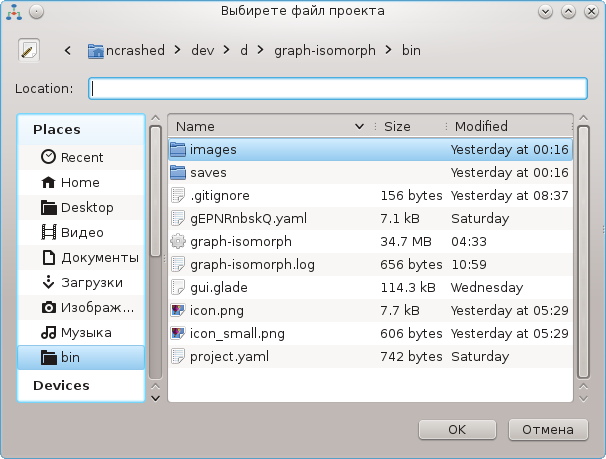
\includegraphics[width=0.7\textwidth]{screen05}
\caption{Диалог открытия файла проекта}
\end{figure}

\begin{figure}[h!]
\centering
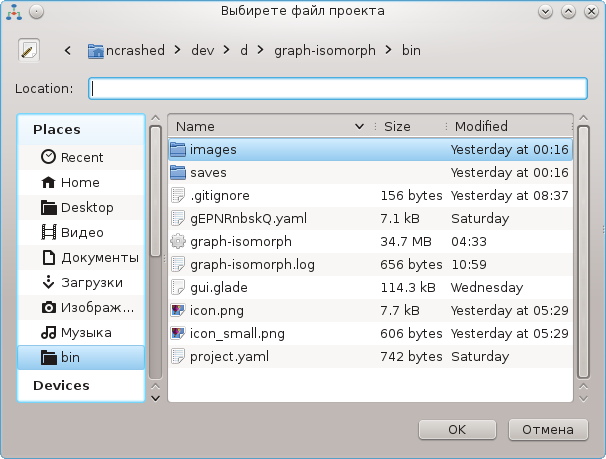
\includegraphics[width=0.7\textwidth]{screen05}
\caption{Ввод параметров эволюционного процесса}
\end{figure}

\subsubsection{Разработка форм выходных данных}

Выходные данные программы отображаются только через графический интерфейс пользователя. Основные виды выходных данных:
\begin{itemize}
\item Названия и описания операторов проблемно-ориентированного языка.
\item Значения параметров эволюционного процесса.
\item Текстовая форма исходного кода найденных алгоритмов. Внутренние структуры проблемно-ориентированного языка преобразуются в человеко-читаемый текст псеводязыка программирования с Си-подобным синтаксисом.
\item Графическая форма исходного кода найденных алгоритмов. Структуры проблемно-ориентированногоя языка преобразовываются в код на языке \textbf{dot} и визуализируются через систему визуализации графов \textbf{Graphviz}.
\end{itemize}


\newpage
\section{Исследовательская часть}

\newpage
\section{Организационно-экономическая часть}
\subsection{Обоснование сметы затрат}
Расчет затрат на разработку данного программного продукта осуществлялся на основе цен за период март-июнь 2014 года.
\subsubsection{Расчет затрат на расходные материалы}
Во время разработки дипломного проекта были произведены следующие затраты на расходные материалы:
\begin{enumerate}
\item Бумага формата А4 с плотностью 80 $\frac{\text{г}}{\text{м}^2}$ 500 листов -- $150$ рубля
\item Печать графической части на формате A1 (11 штук) -- $11 * 50 = 550$ рубля
\item Катридж CE285A для лазерного принтера LaserJet M1132 MFP -- $2670$ рубля
\item Записываемый компакт диск CD-R -- $22$ рубля
\end{enumerate}
Итоговые затраты на расходные материалы: 
$$
C_\text{м} = 3392 \; \text{руб.}
$$

\subsubsection{Расчет затрат на оборудование}
В данном разделе приведены расчеты затрат, связанных с использованием вычислительной техники во время разработки, включая затраты на ремонт данной техники.

Программный продукт разрабатывался на ноутбуке Lenovo IdeaPad V570C 59319588, стоимость которого составляет $14900$ рублей. Конфигурация данного ноутбука является достаточной для разработки и отладки данной системы. Для подготовки документации использовался многофункциональный лазерный принтер LaserJet M1132 MFP стоимостью $5632$ рубля. Итого:
$$
C_\text{об} = 20532 \; \text{руб.}
$$
Длительность использования оборудования: 6 месяцев.

Затраты на вычислительную технику высчитываются по формуле с использованием ускоренных сроков амортизации:
$$
C_\text{эвм} = k \sum_i S_i \frac{T_\text{и}}{12}
$$
Где:
\begin{itemize}
\item $k$ - коэффициент амортизации на год (для ускоренной амортизации k = 0.15 )
\item $\sum_i S_i$ - суммарная стоимость оборудования
\item $T_\text{и}$ - период использования оборудования в месяцах
\end{itemize}

$$
C_\text{эвм} = 0.15 * 20532 * 0.5 = 1539.90 \; \text{руб.}
$$

Таким образом затраты на вычислительную технику при ускоренных сроках амортизации составляют 1539.90 рублей.

Затраты на ремонт вычислительной техники составляют 10\% от ее стоимости:
$$
C_\text{рем} = 0.1 \sum_i S_i = 0.1 * 20532 = 2043.20 \; \text{руб.}
$$
Итоговые затраты на оборудование с учетом ремонта составляют:
$$
C_\text{эвм} + C_\text{рем} = 1539.90 + 2043.20 = 3583.10 \; \text{руб.}
$$

\subsubsection{Расчет затрат на услуги сторонних организаций}
В данном пункте учитываются затраты на выполнение сторонними организациями работ, непосредственно связанных с разработкой данного дипломного проекта.
Затраты на услуги сторонних организаций:
\begin{itemize}
\item Вывод графической части на плоттере с учетом печати черновых листов -- 1100 рублей
\item Переплет программной документации -- 300 рублей
\end{itemize}

Итоговая стоимость услуг сторонних организаций:
$$
C_\text{усо} = 1400 \; \text{руб.}
$$

\subsubsection{Расчет заработной платы}
В данном пункте рассчитывается заработная плата исполнителей, непосредственно связанных с разработкой проекта, с учетом их должностного оклада и времени участия в разработке. 

Затраты на выплату исполнителям заработной платы состоят из двух компонент:
$$
C_\text{зарп} = C_\text{з.осн} + C_\text{з.доп}
$$
Где:
\begin{itemize}
\item $C_\text{з.осн}$ - основная заработная плата
\item $C_\text{з.доп}$ - дополнительная заработная плата
\end{itemize}

Расчет предварительной заработной платы $C_\text{зп}$ производится по следующей формуле:
$$
C_\text{зп} = \sum_{i=1}^n C_\text{minЗП} K_i t_i^\text{РАЗР}
$$
Где:
\begin{enumerate}
\item n - количество работников
\item $C_\text{minЗП}$ - минимальная заработная плата, равная 12600 рублей для жителей Москвы
\item $K_i$ - коэффициент, соответствующий разряду работника, в данном случае равный 1
\item $t_i^\text{РАЗР}$ - время разработки, 6 месяцев
\end{enumerate}
Возможен расчет исходя из трудового договора, где прописан размер заработной платы, который в общем случае может отличаться от нормативной.

$$
C_\text{зп} = 75600 \; \text{руб.}
$$

В соответствии с главой 23 НКРФ доходы физических лиц за вычетом некоторых льгот подлежат обязательному налогообложению (налог на доходы физических лиц). Для компенсации выплат размер  месячного оклада увеличивается, что отражено в формуле:

$$
C_\text{з.осн} = C_\text{зп} (1 + H_\text{дфл}) = 85428 \; \text{руб.}
$$
Где:
\begin{itemize}
\item $C_\text{зп}$ -- сумма к выплате, которая была оговорена с работником
\item $H_\text{дфл}$ -- налог на доходы с физических лиц, 13\%
\end{itemize}


\subsubsection{Расходы на дополнительную заработную плату}
Расходы на дополнительную заработанную плату учитывают все выплаты непосредственно исполнителям за время, не проработанное на производстве, но предусмотренное законодательством, в том числе: оплата очередных отпусков, компенсация за недоиспользованный отпуск, и др. Величина этих выплат составляет 20\% от размера основной заработной платы:	
$$
C_\text{з.доп} = 0.2 C_\text{з.осн} = 17085.60 \; \text{руб.}
$$

В результате получаем:
$$
C_\text{зарп} = C_\text{з.осн} + C_\text{з.доп} = 102513.60 \; \text{руб.}
$$

\subsubsection{Расчет отчислений на социальные нужды}
В данном пункте учитываются отчисления на социальные нужды, производимые в фонды социального страхования, обязательного медицинского страхования и пенсионный фонд. Расчет производится в соответствии с главой 24 Налогового Кодекса РФ «Единый социальный налог (взнос)». 

Ставки единого социального налога определяются в зависимости от величины налогооблагаемой базы. Например, для налоговой базы, рассчитанной для каждого отдельного работника нарастающим итогом с начала года до 624 000 руб., величина единого социального налога рассчитывается по формуле:
$$
C_\text{есн} = K_\text{есн} C_\text{зарп}
$$
Где:
\begin{itemize}
\item $K_\text{есн}$ -- коэффициент отчисления на соц. нужды
\item $C_\text{зарп}$ -- заработная плата в рублях
\end{itemize}

Коэффициент отчислений на социальные нужды без учета льгот складывается из следующих отчислений:
\begin{itemize}
\item ФСС РФ -- отчисление в фонд социального страхования составляет 2.9\% от заработанной платы
\item ПФР -- отчисление в пенсионный фонд составляет 22\%
\item ФФОМС -- отчисление в фонд обязательного медицинского страхования составляет 5.1\%
\end{itemize}

Исходя из приведенной информации:
$$
K_\text{есн} = 0.3
$$
Отсюда:
$$
C_\text{есн} = 30754.08 \; \text{руб.}
$$

Затраты с учетом отчислений на социальные нужды за все время разработки:
$$
C_\text{есн} + C_\text{зарп} = 133267.68 \; \text{руб.}
$$

\subsubsection{Расчет накладных расходов}

В данном пункте учитываются затраты на общехозяйственные расходы, внепроизводственные расходы и расходы на управление.

Накладные расходы составляют 10\% от суммы остальных расходов.

$$
C_\text{нр} = 0.1(C_\text{м} + C_\text{об} + C_\text{усо} + C_\text{зарп} + C_\text{есн}) 
$$
$$
C_\text{нр} = 0.1*(3392 + 20532 + 1400 + 102513.60 + 30754.08) = 15859.17 \; \text{руб.}
$$

\subsubsection{Расчет прочих расходов}
В данном пункте представлены налоги на имущество и налоги на транспортные средства.

Налог на имущество в данном случае не платится, поскольку все имеющееся в наличии имущество, включаемое в налогооблагаемую базу в соответствии с инструкцией «О порядке исчисления и уплаты в бюджет налога на имущество предприятий», используется на нужды образования, и, следовательно, налогом на имущество не облагается.

Налог на владельцев транспортных средств не платится, в связи с отсутствием транспортных средств. 

\subsubsection{Расчет себестоимости}
Себестоимость рассчитывается как сумма по всем выше перечисленным статьям затрат и составляет:
$$
S = C_\text{нр} + C_\text{м} + C_\text{об} + C_\text{усо} + C_\text{проч} + C_\text{зарп} + C_\text{есн} = 174450.85 \; \text{руб.}
$$

\subsubsection{Расчет прибыли}
Расчет прибыли ведется с учетом отчислений в местный бюджет и налога на прибыль. Отчисления в местный бюджет составляют 4.5\% от себестоимости и равны 6978.03 рублей. Чистая прибыль составляет 10\% от себестоимости и равна 17445.09 рублей. Налог на прибыль составляет 35\% и равен 61057.80 рублей.

Итого:
$$
P = 6978.03 + 17445.09 + 61057.80 = 85480.92 \; \text{руб}
$$

\subsubsection{Цена (без НДС)}
Цена программного продукта определяется путем суммирования прибыли и себестоимости и составляет: 
$$
\text{Ц} = P + S = 174450.85 + 85480.92 = 259931.77  \; \text{руб}
$$

\subsubsection{Цена (с НДС)}
В виду того, что реализация товаров и услуг на территории РФ осуществляется с налогом на добавленную стоимость (18\% от цены), в цену изделия включается НДС. Тогда окончательная цена разработанной системы с учетом НДС составляет:
$$
\text{Ц}_\text{ндс} = \text{Ц}(1 + 0.18) = 259931.77*1.18 = 306719.49 \; \text{руб}
$$

\subsection{Эргономика рабочего места и организация рабочего пространства}
Говоря об эргономике в компьютерной области, можно сказать, что это достаточно молодая сфера. Бурное развитие она приобрела за последние десять лет. И по мере компьютеризации человечества она становится все более актуальной. Ведь согласитесь, что сейчас пользователи проводят за компьютерами намного больше времени, чем когда-либо. А незнание и невыполнение правил работы с ним часто оборачивается не только плохим самочувствием, но и потерей здоровья. 

Трудовая активность человека во многом определяется условиями, в которых он работает. К ним прежде всего относятся рабочее пространство и рабочее место. Та часть рабочего пространства, гед располагается производственное оборудование, с которым взаимодействует человек в рабочей среде, называется рабочим местом \cite{Ergonomic}.

Как показали научные исследования, однообразные движения, совершаемые в течение длительного времени, в сочетании с плохой организацией труда и рабочего места вызывают физические неудобства и наносят вред здоровью. Чаще всего возникают воспалительные заболевания сухожилий. 
Неправильная организация рабочего места может вызвать ненужную нагрузку на мышцы. Исследования показали, что примерно 20\% нарушений, связанных с работой за компьютером, вызваны неправильной организацией рабочего места. 

Хорошая организация рабочего пространства очень важна для сохранения здоровья, поэтому необходимо ответить на несколько вопросов, ответы на которые должны помочь организовать его.

\subsubsection{Как будет использоваться ЭВМ}

\paragraph{Кто будет работать за ним?}

Если за компьютером работает только один человек, то рабочее пространство заранее можно оптимально организовать под этого человека. И, например регулировка стула по высоте может не являться необходимостью. При работе нескольких человек за одним компьютером рабочее место должно подстраиваться под каждого человека, и чем больше различия между людьми, тем более широкий диапазон регулировки рабочего места необходим. Для того, чтобы обеспечить максимально комфортные условия каждому.

\paragraph{Как долго предполагается использовать компьютер в течение дня?}

Если компьютер используется несколько минут в день (до 30 минут), то вопросы эргономичной организации пространства не являются первостепенными. Если компьютер используется более 1 часа, то следует уделить достаточное внимание организации рабочего места. И если компьютер используется больше 4 часов, следует максимально обдуманно организовать рабочее место. 

Необходимо определить, какого типа программы будут работать на компьютере чаще всего. В зависимости от этого следует перед собой расположить, то устройства ввода, с которым приходится работать чаще всего.

\paragraph{Текстовые редакторы}
Удобное расположение клавиатуры с мышью наиболее важно. Современные клавиатуры имеют с правой стороны цифровую панель, поэтому при печатании текста, алфавитный набор клавиш нужно расположить перед собой по центру, для этого клавиатуру нужно сдвинуть немного вправо, так, чтобы клавиша с латинской буквой В попадала на центральную линию тела. Последние исследования в области эргономики показали, что идеальное положение при наборе текста, когда клавиатура находится под наклоном, такое положения может обеспечить специальный регулируемый держатель для клавиатуры.

\subsubsection{Помещение и освещение}
В помещении, предназначенном для работы на компьютере, должно иметься как естественное, так и искусственное освещение. Лучше всего, если окна в комнате выходят на север или северо-восток. Помещения необходимо оборудовать не только отопительными приборами, но и системами кондиционирования воздуха или эффективной вентиляцией. Стены и потолки следует окрашивать матовой краской: блестящие и тем более, зеркальные поверхности утомляют зрение и отвлекают от работы. В помещениях ежедневно должна проводиться влажная уборка.

Желательно, чтобы площадь рабочего места составляла не менее 6 квадратных метров, а объем - 20 кубических метров. Стол следует поставить сбоку от окна так, чтобы свет падал слева. Наилучшее освещение для работы с компьютером - рассеянный непрямой свет, который не дает бликов на экране. В поле зрения пользователя не должно быть резких перепадов яркости, поэтому окна желательно закрывать шторами либо жалюзи. Искусственное же освещение должно быть общим и равномерным, в то же время использование одних только настольных ламп недопустимо.

\subsubsection{Организация рабочего стола}

На рабочем столе должны свободно помещаться монитор, клавиатура, мышь и другое компьютерное оборудование, а также документы, книги, бумаги - все необходимые для работы вещи. Если вы хотите разместить в ряд несколько столов с мониторами, то следует поставить их таким образом, чтобы расстояние в ряду составляло не менее 2 метров, а между рядами - 1,2 метра. Врачи полагают, что при выполнении творческой работы, требующей значительного умственного напряжения или высокой концентрации внимания, рабочие места желательно изолировать друг от друга перегородками высотой 1,5-2 метра.

Помимо вышесказанного, строгие требования должны предъявляться к стулу, который просто необходим для поддержки правильной позы с учетом особенностей фигуры и изменения ее для снижения статического напряжения мышц шейно-плечевой области и спины. Желательно, чтобы стул регулировался по высоте, углам наклона сиденья и спинки, а также по расстоянию спинки от переднего края сиденья. Поверхности сиденья, спинки и подлокотников должны быть полумягкими, с покрытием, которое не скользит, не электризуется и пропускает воздух.

К сожалению, часто при работе очень мало внимания уделяется этому аспекту.

\subsubsection{Правильная высота}
Чтобы определить наиболее подходящую высоту стула, сядьте на него и положите руки на клавиатуру: ноги должны полностью касаться пола, бедра - находиться немного выше колен, спина - чувствовать упор, а предплечья - быть параллельными полу. Монитор следует размещать на столе прямо перед собой примерно на расстоянии вытянутой руки так, чтобы верхняя граница монитора находилась на уровне глаз или ниже не более чем на 15 сантиметров. 

Правильное положение рук при работе с клавиатурой и мышью: локти располагаются параллельно поверхности стола и под прямым углом к плечу. Запястья не должны быть согнутыми, иначе возможно их повреждение. Желательно, чтобы во время работы запястья на что-нибудь опирались. Конструкция современных клавиатур и мышей предусматривает для них опору (дизайн клавиатуры и специальные коврики). Однако вы легко можете сами изготовить ее, например, взяв узкую полоску пенопласта и положив ее перед клавиатурой или мышью (однако следует учитывать, чтобы материал не вызывал чрезмерного раздражения рецепторов кожи (аллергические реакции), что может привести к возникновению заболеваний кожи). Клавиатура должна располагаться в 10-15 сантиметрах от края стола.

\subsubsection{Эргономичная мебель}
Разработанные медиками санитарно-гигиенические нормы должны учитываться при конструировании компьютерной и офисной мебели, а также при проектировании помещений офисов. В последнее время изделия, изготовленные с учетом требований гигиены и комфорта, часто называют эргономичными. Эргономика - наука о взаимодействии человека и машины. Сегодня одна из главных ее задач - снизить нагрузки на организм человека, связанные с работой на компьютере. Так, например, "эргономичная мышь" сконструирована таким образом, чтобы поддерживать запястье в нужном положении. Очевидно, одно из главных требований к современной компьютерной мебели - ее эргономичность.

Что представляет собой компьютерная мебель сегодня? Это чаще всего так называемая "универсальная стойка для компьютерного оборудования". Она, как правило, представляет собой подставку для монитора, "скворечник" для процессорного блока и полочку для принтера. Основные достоинства такой стойки - низкая цена и компактность, что немаловажно для небольших квартир.

В офисах компьютеры часто размещают на больших столах с выдвижной доской для клавиатуры. Монитор обычно ставят на угол, и во время работы все время приходится смотреть вправо или влево. Можно создать более удобную рабочую обстановку - соорудить Г-образный стол, то получите более удобный доступ к материалам. 

Отдельной критики заслуживают выдвижные полки для клавиатуры. Как показали исследования, профессиональная болезнь машинисток (синдром запястного канала) зачастую вызвана именно этим приспособлением. Это неудивительно: высота офисного стола рассчитана на письменные работы, и клавиатура на выдвижной подставке оказывается заведомо ниже нормы.
\subsubsection{Вентиляция}

Рабочее место должно быть с хорошей вентиляцией. С одной стороны это важно для охлаждения разных частей компьютера, который выделяют тепло в процессе работы (системный блок, монитор, принтер и т.п.), а с другой стороны приток свежего воздуха в достаточной мере снабжает организм кислородом.

Если Вы курите, ни в коем случае не курите за компьютером, курение за компьютером только дополнительно дает нагрузку на Ваш организм. В результате курения в крови накапливается вредный монооксид углерода (СО), а это снижает способность организма обеспечивать кровоснабжение мышц. Курение также снижает прочность соединительной ткани в мышцах, увеличивая вероятность их травмирования.

\subsubsection{Шум}

Шум на рабочем месте может быть причиной стресса и вызывать лишнее напряжение мышц, что в свою очередь повышает утомляемость организма и снижает работоспособность. Поэтому необходимо выбирать по возможности тихое место. Используйте негромкое музыкальное сопровождение в качестве фона, для того чтобы замаскировать шум вентиляторов, винчестеров, принтера и т.п. 

\subsubsection{Рабочее кресло}

Какой стул следует принимать на рабочем месте? Всем известно, что продолжительная сидячая работа вредна человеку, поэтому удобное рабочее кресло - это и наше здоровье, и настроение, и работоспособность, и производительность. Как говорит "всезнающая" статистика: работа на эргономически правильно сконструированных стульях по сравнению с обычными стульями:
\begin{itemize}
\item уменьшает число ошибок в два раза
\item повышает концентрацию внимания (+ 7\%)
\item сохраняет активность (+ 9\%)
\item сохраняет позитивное самочувствие (+ 15\%)
\item способствует хорошему настроению (+ 10\%)
\end{itemize}

Необходимо, чтобы рабочий стул свободно вращался относительно основания, регулировался по высоте и, кроме того, допускал возможность изменять угол наклона спинки (хорошо, если и сиденья тоже), а также устанавливать нужное расстояние от спинки до переднего края сиденья. Обивка кресла должна быть не только практичной, стойкой к длительным физическим воздействиям, но и гигиеничной, т. е. выполненной из материалов, безвредных для здоровья и обеспечивающих удобство и комфорт в работе.

Идеальная высота сиденья - когда ступни ног полностью касаются пола, а угол сгиба коленей при этом составляет примерно 90 градусов. Очень важно, чтобы край сиденья имел мягкую скругленную вниз форму. Это позволяет избежать давления на кровеносные сосуды и не нарушать циркуляцию крови.

Позвоночник здорового человека напоминает знак интеграла. А, следовательно, спинке кресла необходимо иметь соответствующую форму, чтобы помогать сохранять это положение. Это очень важный момент. Если приходится сидеть на обычном стуле без выпуклости под поясницу, рекомендуется применять небольшую мягкую подушку для этих целей. Угол между спинкой кресла и сидением должен составлять чуть более 90 градусов. Иногда стулья снабжаются специальным механизмом, позволяющим одновременно менять угол наклона спинки и сиденья так, что положение позвоночника остается правильным в любой момент времени.

Хорошо, если спинка стула поддерживает лишь нижнюю половину спины, но при этом не является жестко закрепленной, чтобы не препятствовать движениям в процессе работы. 

\subsubsection{Как следует сидеть за ЭВМ}

\textbf{Осанка} - это положение, которое принимает ваше тело, когда вы сидите за компьютером.

Правильная осанка необходима для профилактики заболеваний шеи, рук, ног и спины. Необходимо так организовать свое рабочее место, чтобы осанка была оптимальной.

\paragraph{Правильная осанка}
Старайтесь сидеть за компьютером на 2,5 см выше, чем обычно. 

Расположите монитор прямо перед собой. Верхняя треть экрана - на уровне глаз, чтобы при работе угол наклона шеи был естественным. 

Настройте высоту спинки стула таким образом, чтобы она соприкасалась с местом наибольшего изгиба спины. 

Уши должны располагаться точно в плоскости плеч. 

Плечи должны располагаться точно над бедрами. 

Когда вы смотрите вниз, голова должна находиться точно над шеей, а не наклоняться вперед. 

Опирайтесь обеими ступнями о пол или подставку для ног. Под столом должно быть достаточно просторно, чтобы Вы свободно могли вытягивать ноги. 

Руки должны удобно располагаться по сторонам. 

Локти согнуты и находятся примерно в 3 см от корпуса. 

Запястья должны принять нейтральное положение (ни подняты, ни опущены). 

Сядьте так, чтобы край стула не давил под колени. 

Правильная осанка во время работы максимально разгружает мышцы и позволяет работать дольше, меньше уставая. 

Но даже абсолютно правильная осанка не поможет, если весь день сидеть в одной позе. Неподвижное положение, даже абсолютно правильное, приведет к мышечной усталости. 

Правильная осанка предусматривает изменение позы примерно дважды в час. 

Длительное пребывание в одной и той же позе заставляет мышцы работать непрерывно без отдыха. Из-за отсутствия достаточного отдыха или изменения позы в мышцах накапливаются продукты распада, вызывающие болезненные ощущения. Для удаления продуктов распада и питания мышц необходимо адекватное кровоснабжение. Даже незначительное изменение положения тела каждые полчаса смещает нагрузку на другие мышцы, что позволяет мышцам отдыхать и запасаться питательными веществами. 

\paragraph{Типичные нарушения осанки во время работы}
\textbf{Вытягивание шеи} вперед приводит к напряжению мышц шеи, что может в свою очередь привести к сдавливанию уходящих в голову нервов, и это вызовет боль. Эта поза увеличивает нагрузку на мышцы шеи в три раза. Мышцы шеи, поддерживающие голову, удлиняются, что может приводить к сдавливанию нерва.

Эта вредная привычка (вытягивать шею) может быть обусловлена тем, что монитор отодвинут слишком далеко. В результате, работающий на компьютере вытягивает шею вперед, чтобы лучше увидеть экран \cite{Shilova}.

\textbf{Сутулые плечи} вызывают сдавливание сухожилий передней поверхности плеча, что приводит к боли в области руки и плеча.

Для того чтобы в течение дня поддерживать правильную осанку, мышцам, которые за это отвечают, необходим отдых. Это - мышцы спины, шеи и живота. Они должны получать кровоснабжение, достаточное для того, чтобы обеспечивать вертикальное положение головы и прямую спину в течение дня. Сильные мышцы помогают сохранять правильную осанку в течение более длительных периодов времени и повышают продуктивность работы. 

\paragraph{О труде и отдыхе}
Но и правильная осанка, и хорошая мебель не помогут \cite{Shilova}, если весь день сидеть в одной позе. Длительное неподвижное положение приведет к мышечной усталости. Если вам приходится весь день сидеть, вставайте время от времени либо слегка изменяйте высоту кресла или крышки стола, чтобы изменить общее положение тела.
Согласно требованиям, разработанным Госсанэпиднадзором, суммарное время непосредственной работы с персональным компьютером не должно превышать шести часов за смену. На протяжении рабочего дня следует устраивать перерывы продолжительностью 10 - 20 минут. Работа без перерыва за монитором компьютера не должна превышать 45 - 60 минут. Во время перерывов рекомендуется выполнять необходимые комплексы физических упражнений.

\newpage
\section{Заключение}
В результате выполнения задания на курсовое проектирование была получен инструмент для решения актуальной задачи. Результаты работы данной АИС могут быть применены в различных областях, но самым интересным практическим применением является сопоставление знаний в двух разных семантических сетях. Возникновение необходимости решать задачи такого рода являлось предпосылкой к созданию данного инструментарного средства.

Хотя данный программный продукт и производит поиск алгоритмов решения задачи проверки изоморфизма ориентированных графов, система может и найти решение за приемлимые временные рамки, так как метод генетического программирования не гарантирует нахождение оптимального решения за конечное количство обработанных поколений. Также решение может быть не найдено, так как исходная задача может принадлежать к классу NP-полных задач, однако это не доказано. Главное преимущество метода генетического программирования - возможность поиска по всему пространству возможных решений, не привлекая при этом человеческие интеллектуальные ресурсы.

В ходе выполнения курсового проектирования была изучена предметная область, изучен метод генетического программирования сложных алгоритмов, разобраны нюансы разработки проблемно-ориентированных языков и интерпретаторов, углублены знания в проектировании крупных программных продуктов, создании технической документации, создании схем UML. Были использованы современные технологии такие, как: язык программирования D, операционная система семейства GNU/Linux, графический интерфейс на основе GTK+, распределенные система контроля версий Git и система компьютерной верстки \TeX.

\newpage
%\addcontentsline{toc}{chapter}{\bibname}
\bibliographystyle{utf8gost705u}  %% стилевой файл для оформления по ГОСТу
\bibliography{biblio}     %% имя библиографической базы (bib-файла) 

\end{spacing}
\end{document}